% This is the Reed College LaTeX thesis template. Most of the work
% for the document class was done by Sam Noble (SN), as well as this
% template. Later comments etc. by Ben Salzberg (BTS). Additional
% restructuring and APA support by Jess Youngberg (JY).
% Your comments and suggestions are more than welcome; please email
% them to cus@reed.edu
%
% See http://web.reed.edu/cis/help/latex.html for help. There are a
% great bunch of help pages there, with notes on
% getting started, bibtex, etc. Go there and read it if you're not
% already familiar with LaTeX.
%
% Any line that starts with a percent symbol is a comment.
% They won't show up in the document, and are useful for notes
% to yourself and explaining commands.
% Commenting also removes a line from the document;
% very handy for troubleshooting problems. -BTS

% As far as I know, this follows the requirements laid out in
% the 2002-2003 Senior Handbook. Ask a librarian to check the
% document before binding. -SN

%%
%% Preamble
%%
% \documentclass{<something>} must begin each LaTeX document
\documentclass[12pt,twoside]{reedthesis}
% Packages are extensions to the basic LaTeX functions. Whatever you
% want to typeset, there is probably a package out there for it.
% Chemistry (chemtex), screenplays, you name it.
% Check out CTAN to see: http://www.ctan.org/
%%
\usepackage{graphicx,latexsym}
\usepackage[french]{babel} 
\usepackage{amsmath}
\usepackage{amssymb,amsthm}
\usepackage{xcolor}
\usepackage{eso-pic}
\usepackage{longtable,booktabs,setspace}
\usepackage{chemarr} %% Useful for one reaction arrow, useless if you're not a chem major
\usepackage[hyphens]{url}
\usepackage{pdfpages}
\usepackage{tikz}
\usetikzlibrary{calc}
\newcommand\HRule{\rule{\textwidth}{1pt}}
% Added by CII
\usepackage{hyperref}
\usepackage{lmodern}
\usepackage{float}
\floatplacement{figure}{H}
% End of CII addition
\usepackage{rotating}

% Next line commented out by CII
%%% \usepackage{natbib}
% Comment out the natbib line above and uncomment the following two lines to use the new
% biblatex-chicago style, for Chicago A. Also make some changes at the end where the
% bibliography is included.
%\usepackage{biblatex-chicago}
%\bibliography{thesis}

% Added by CII (Thanks, Hadley!)
% Use ref for internal links
\renewcommand{\hyperref}[2][???]{\autoref{#1}}
\def\chapterautorefname{Chapter}
\def\sectionautorefname{Section}
\def\subsectionautorefname{Subsection}
% End of CII addition

% Added by CII
\usepackage{caption}
\captionsetup{width=5in}
% End of CII addition

% \usepackage{times} % other fonts are available like times, bookman, charter, palatino

% To pass between YAML and LaTeX the dollar signs are added by CII
\title{THÈSE}
\author{Keurcien LUU}
\labo{Techniques de l'Ingénierie Médicale et de la Complexité - Informatique,
Mathématiques et Applications de Grenoble (TIMC-IMAG)}
% The month and year that you submit your FINAL draft TO THE LIBRARY (May or December)
\date{31 octobre 2017}
\division{Mathematics and Natural Sciences}
\advisor{Michael BLUM}
%If you have two advisors for some reason, you can use the following
% Uncommented out by CII
% End of CII addition

%%% Remember to use the correct department!
\department{Ingénierie de la Santé, de la Cognition et Environnement (EDISCE)}
% if you're writing a thesis in an interdisciplinary major,
% uncomment the line below and change the text as appropriate.
% check the Senior Handbook if unsure.
%\thedivisionof{The Established Interdisciplinary Committee for}
% if you want the approval page to say "Approved for the Committee",
% uncomment the next line
%\approvedforthe{Committee}

% Added by CII
%%% Copied from knitr
%% maxwidth is the original width if it's less than linewidth
%% otherwise use linewidth (to make sure the graphics do not exceed the margin)
\makeatletter
\def\maxwidth{ %
  \ifdim\Gin@nat@width>\linewidth
    \linewidth
  \else
    \Gin@nat@width
  \fi
}
\makeatother

\renewcommand{\contentsname}{Table of Contents}
% End of CII addition

\setlength{\parskip}{0pt}

% Added by CII

\providecommand{\tightlist}{%
  \setlength{\itemsep}{0pt}\setlength{\parskip}{0pt}}

\Acknowledgements{
The preface pretty much says it all. \par  Second paragraph of abstract
starts here.
}

\Dedication{

}

\Preface{
The preface pretty much says it all. \par
}

\Abstract{
The preface pretty much says it all. \par  Second paragraph of abstract
starts here.
}

% End of CII addition
%%
%% End Preamble
%%
%

\begin{document}

% Everything below added by CII
      \maketitle
  
  \frontmatter % this stuff will be roman-numbered
  \pagestyle{empty} % this removes page numbers from the frontmatter

      \begin{acknowledgements}
      The preface pretty much says it all. \par  Second paragraph of abstract
      starts here.
    \end{acknowledgements}
  
      \begin{preface}
      The preface pretty much says it all. \par
    \end{preface}
  
      \hypersetup{linkcolor=black}
    \setcounter{tocdepth}{2}
    \tableofcontents
  
      \listoftables
  
      \listoffigures
  
      \begin{abstract}
      The preface pretty much says it all. \par  Second paragraph of abstract
      starts here.
    \end{abstract}
  
  
  \mainmatter % here the regular arabic numbering starts
  \pagestyle{fancyplain} % turns page numbering back on

  \chapter*{Introduction}\label{introduction}
  \addcontentsline{toc}{chapter}{Introduction}
  
  « Je me propose de passer brièvement en revue les progrès de l'opinion
  relativement à l'origine des espèces. Jusque tout récemment, la plupart
  des naturalistes croyaient que les espèces sont des productions
  immuables créées séparément. De nombreux savants ont habilement soutenu
  cette hypothèse. Quelques autres, au contraire, ont admis que les
  espèces éprouvent des modifications et que les formes actuelles
  descendent de formes préexistantes par voie de génération régulière. »
  
  C'est de cette manière qu'en 1920, Edmond Barbier, dans sa notice
  relative à la traduction française de \textit{L'Origine des espèces}
  (Darwin, 1980), décide de présenter le contexte dans lequel il a été
  amené à effectuer ce travail de traduction. Ce constat qu'il partage,
  réalisé il y a presque cent ans, semble pourtant valoir encore
  aujourd'hui. Si bien que chaque sortie de l'Église catholique affirmant
  la compatibilité entre la religion et la théorie évolutionniste apporte
  son lot de débats et de controverses.
  
  \section{Qu'est-ce que la génétique ?}\label{quest-ce-que-la-genetique}
  
  À cette question nous pourrions reprendre en guise de réponse la
  formulation de Cavalli-Sforza, traduite de l'italien (Cavalli-Sforza,
  1994): « La génétique est la science de l'hérédité. Elle est la clé de
  toute la biologie, parce qu'elle explique les mécanismes qui sont
  responsables de la reproduction des êtres vivants, du fonctionnement et
  de la transmission du matériel héréditaire, des différences entre les
  individus, de l'évolution biologique. »
  
  \section{Données en grande dimension}\label{donnees-en-grande-dimension}
  
  L'accumulation de données, aussi bien en termes d'observations qu'en
  termes de variables, laisse à penser que le traitement de celles-ci
  pourrait permettre de détecter efficacement les variables qui sont
  responsables ou qui influencent un phénomène particulier. Cela pourrait
  être par exemple l'utilisation de bases de données automobiles pour
  prédire la durée de vie de véhicules neufs, ou encore celle de données
  climatiques pour estimer les variations de température auxquelles
  pourrait être sujette notre planète. Cette accumulation massive
  s'accompagne tout de même d'un phénomène bien connu en statistiques,
  phénomène qui porte le nom de ``curse of dimensionality'' (Giraud,
  2014).
  
  Dérive génétique Environnement hétérogène
  
  \chapter{État de l'art}\label{etat-de-lart}
  
  \section{L'indice de fixation}\label{lindice-de-fixation}
  
  En se différenciant génétiquement, les populations voient leurs
  fréquences d'allèles évoluer de façon indépendante. L'indice de fixation
  est une statistique permettant de quantifier pour un allèle donné,
  l'écart de la fréquence observée dans une sous-population à la fréquence
  théorique
  
  \section{Modèle de FLK}\label{modele-de-flk}
  
  Le modèle de FLK estime le modèle neutre d'un SNP bi-allélique lorsque
  celui-ci est uniquement soumis à la dérive génétique. À l'instant
  \(t = 0\), le SNP a une fréquence \(p_0\). Notant \(F_t\) l'indice de
  fixation de cet allèle, \(p(t)\) sa fréquence après \(t\) générations,
  et en supposant que \(F_t\) soit suffisamment petit, ce qui devrait être
  vérifié dans le cas neutre. (Nicholson et al., 2002) :
  
  \begin{equation} 
    p(t) \sim N(p_0, F_t p_0 (1-p_0)) 
    \label{eq:frequency-law}
  \end{equation}
  
  De la loi \eqref{eq:frequency-law} nous tirons
  \(\text{Var}(p(t)) = F_t p_0 (1-p_0)\).
  
  La statistique FLK (Bonhomme et al., 2010) requiert d'estimer au
  préalable deux paramètres que sont la fréquence allélique initiale
  \(p_0\) et la matrice d'apparentement \(V\), \(V \in M_K(\mathbb{R})\)
  où \(K\) est le nombre de populations observées. Notant :
  
  \begin{itemize}
  \item
    \(\boldsymbol{p} = (p_1, p_2, \dots, p_K) \in \mathbb{R}^K\),
  \item
    \(\boldsymbol{p_0} = (p_0, p_0, \dots, p_0) \in \mathbb{R}^K\),
  \item
    \(\boldsymbol{r} = N(0, V)\),
  \end{itemize}
  
  le modèle neutre pour \(\boldsymbol{p}\) est donné par la relation
  suivante :
  
  \begin{equation} 
    \boldsymbol{p} = \boldsymbol{p_0} + \boldsymbol{r} 
    \label{eq:flk_neutral_model}
  \end{equation}
  
  Bonhomme \textit{et al.} proposent pour ce modèle de mesurer une
  statistique de qualité de l'ajustement pour quantifier la déviance d'un
  allèle par rapport au modèle neutre :
  
  \begin{equation} 
    FLK = (\boldsymbol{p - \hat{p}_0})^T V (\boldsymbol{p - \hat{p}_0})                                \label{eq:flk-statistic}
  \end{equation}
  
  Sous l'hypothèse neutre et suivant \eqref{eq:flk-statistic},
  \(FLK \sim \chi^2 (K - 1)\).
  
  \section{Modèle de OutFLANK}\label{modele-de-outflank}
  
  En reprenant le modèle proposé par Lewontin et Krakauer (Lewontin \&
  Krakauer, 1973) et en y apportant les corrections nécessaires afin de
  prendre en compte les erreurs d'échantillonnage, Whitlock
  \textit{et al.} proposent une méthode permettant de détecter les allèles
  sous sélection en environnement hétérogène (Whitlock \& Lotterhos,
  2015). Ainsi, la quantité
  
  \begin{equation} 
    k \frac{F_{ST}^{\prime}}{\bar{{F_{ST}^{\prime}}}}  
    \label{eq:OutFLANK-statistic}
  \end{equation}
  
  où \(k\) représente le nombre de degrés de libertés.
  
  \section{Modèle du logiciel Bayescan}\label{modele-du-logiciel-bayescan}
  
  Bayescan est aujourd'hui encore un des logiciels les plus utilisés pour
  détecter l'adaptation locale. Le modèle employé suppose que les
  sous-populations observées proviennent toutes d'une même population
  ancestrale. Pour une sous-population donnée et un SNP donné, la
  statistique de \(F_{ST}\) peut être estimée en utilisant la
  vraisemblance d'un modèle multinomial-Dirichlet (Beaumont \& Balding,
  2004). \(F_{ST} \in [0, 1]\) est une quantité qui peut être interprété
  comme proportionnel à la probabilité que deux individus aient un ancêtre
  commun dans la sous-population
  
  \begin{equation} 
    \log \left( \frac{F_{ST}}{1 - F_{ST}} \right) = \alpha_j + \beta_i + \gamma_{ij}
    \label{eq:Bayescan-statistic}
  \end{equation}
  
  \section{Fast PCA}\label{fast-pca}
  
  \begin{itemize}
  \tightlist
  \item
    ACP en génétique des populations
  \end{itemize}
  
  \section{Analyse en Composantes Principales
  parcimonieuse}\label{analyse-en-composantes-principales-parcimonieuse}
  
  \section{Bootstrap ACP}\label{bootstrap-acp}
  
  \section{Contexte}\label{contexte}
  
  \section{Tests multiples}\label{tests-multiples}
  
  \section{Contrôle du taux de fausse
  découverte}\label{controle-du-taux-de-fausse-decouverte}
  
  Le taux de fausse découverte, correspond à la proportion de faux
  positifs parmi les positifs. En notant \(FP\) le nombre de faux
  positifs, \(FP\) le nombre de vrais positifs, on définit le taux de
  fausse découverte \(FDR\) par :
  \[ FDR = \mathbb{E}\Big[\frac{FP}{TP + FP} 1_{FP+TP > 0}\Big] \] -
  Référence cours de Christophe Giraud
  
  q-value, bonferroni, benjamini-hochberg La figure suivante donne les
  comparaisons entre les différentes procédures de correction :
  
  \chapter{Adaptation locale}\label{adaptation-locale}
  
  Une population est dite localement adaptée à son environnement si elle a
  connu une évolution différente de celles qu'ont connu les autres
  populations de la même espèce, et ce, en réponse aux pressions
  sélectives auxquelles elle peut être confrontrée.
  
  \section{Cas d'étude utilisant
  pcadapt}\label{cas-detude-utilisant-pcadapt}
  
  \section{Simulations et modèles
  démographiques}\label{simulations-et-modeles-demographiques}
  
  \subsection{Modèle en île}\label{modele-en-ile}
  
  \subsection{Modèle de divergence}\label{modele-de-divergence}
  
  Nous adaptons une version du script Python utilisé dans (Roux et al.,
  2012), basé sur le module de simulation simuPOP (Peng \& Kimmel, 2005).
  
  \begin{Shaded}
  \begin{Highlighting}[]
  \CommentTok{#!/usr/bin/env python}
  \ImportTok{from} \NormalTok{__future__ }\ImportTok{import} \NormalTok{division}
  \ImportTok{import} \NormalTok{simuOpt, types, os, sys, time}
  \NormalTok{simuOpt.setOptions(alleleType }\OperatorTok{=} \StringTok{'long'}\NormalTok{)}
  \ImportTok{from} \NormalTok{operator }\ImportTok{import} \NormalTok{itemgetter}
  \ImportTok{import} \NormalTok{numpy }\ImportTok{as} \NormalTok{np}
  \ImportTok{from} \NormalTok{simuPOP }\ImportTok{import} \OperatorTok{*}
  \ImportTok{from} \NormalTok{simuPOP.utils }\ImportTok{import} \OperatorTok{*}
  \ImportTok{from} \NormalTok{simuPOP.sampling }\ImportTok{import} \NormalTok{drawRandomSample}
  
  \KeywordTok{def} \NormalTok{simulate(Ne, Nsam, T1, T2, T3, s10, s11):}
      \NormalTok{pop }\OperatorTok{=} \NormalTok{Population(size }\OperatorTok{=} \NormalTok{Ne, }
                       \NormalTok{ploidy }\OperatorTok{=} \DecValTok{2}\NormalTok{, }
                       \NormalTok{loci }\OperatorTok{=} \NormalTok{[}\DecValTok{1}\NormalTok{], }
                       \NormalTok{infoFields }\OperatorTok{=} \NormalTok{[}\StringTok{'fitness'}\NormalTok{, }\StringTok{'migrate_to'}\NormalTok{])}
                       
      \KeywordTok{def} \NormalTok{getfitness10(geno):}
          \ControlFlowTok{if} \NormalTok{geno[}\DecValTok{0}\NormalTok{] }\OperatorTok{+} \NormalTok{geno[}\DecValTok{1}\NormalTok{] }\OperatorTok{==} \DecValTok{0} \NormalTok{:}
              \ControlFlowTok{return} \DecValTok{1} \OperatorTok{-} \DecValTok{2} \OperatorTok{*} \NormalTok{s10}
          \ControlFlowTok{if} \NormalTok{geno[}\DecValTok{0}\NormalTok{] }\OperatorTok{+} \NormalTok{geno[}\DecValTok{1}\NormalTok{] }\OperatorTok{==} \DecValTok{1} \NormalTok{:}
              \ControlFlowTok{return} \DecValTok{1} \OperatorTok{-} \NormalTok{s10}
          \ControlFlowTok{else} \NormalTok{:}
              \ControlFlowTok{return} \DecValTok{1}
  
      \KeywordTok{def} \NormalTok{getfitness11(geno):}
          \ControlFlowTok{if} \NormalTok{geno[}\DecValTok{0}\NormalTok{] }\OperatorTok{+} \NormalTok{geno[}\DecValTok{1}\NormalTok{] }\OperatorTok{==} \DecValTok{0} \NormalTok{:}
              \ControlFlowTok{return} \DecValTok{1} \OperatorTok{-} \DecValTok{2} \OperatorTok{*} \NormalTok{s11}
          \ControlFlowTok{if} \NormalTok{geno[}\DecValTok{0}\NormalTok{] }\OperatorTok{+} \NormalTok{geno[}\DecValTok{1}\NormalTok{] }\OperatorTok{==} \DecValTok{1} \NormalTok{:}
              \ControlFlowTok{return} \DecValTok{1} \OperatorTok{-} \NormalTok{s11}
          \ControlFlowTok{else} \NormalTok{:}
              \ControlFlowTok{return} \DecValTok{1}
              
      \NormalTok{pop.evolve( }
          \NormalTok{initOps }\OperatorTok{=} \NormalTok{[}
              \NormalTok{InitSex(),}
              \NormalTok{InitGenotype(loci }\OperatorTok{=} \NormalTok{ALL_AVAIL, }
                           \NormalTok{freq }\OperatorTok{=} \NormalTok{[}\FloatTok{0.5}\NormalTok{, }\FloatTok{0.5}\NormalTok{],  }
                           \NormalTok{begin }\OperatorTok{=} \DecValTok{0}\NormalTok{, }
                           \NormalTok{end }\OperatorTok{=} \DecValTok{1}\NormalTok{)}
          \NormalTok{],}
          
          \NormalTok{preOps }\OperatorTok{=} \NormalTok{[}
              \CommentTok{# resize the ancestral population at the time immediatly }
              \CommentTok{# before the split}
              \NormalTok{ResizeSubPops([}\DecValTok{0}\NormalTok{], }
                            \NormalTok{sizes }\OperatorTok{=} \NormalTok{[Ne }\OperatorTok{+} \NormalTok{Ne], }
                            \NormalTok{at }\OperatorTok{=} \NormalTok{T1 }\OperatorTok{-} \DecValTok{1}\NormalTok{),}
                                
              \NormalTok{ResizeSubPops([}\StringTok{"S1_1"}\NormalTok{], }
                            \NormalTok{sizes }\OperatorTok{=} \NormalTok{[Ne }\OperatorTok{+} \NormalTok{Ne], }
                            \NormalTok{at }\OperatorTok{=} \NormalTok{T1 }\OperatorTok{+} \NormalTok{T2 }\OperatorTok{-} \DecValTok{1}\NormalTok{),}
                                
              \CommentTok{# split populations in 2 subpopulations }
              \NormalTok{SplitSubPops(subPops }\OperatorTok{=} \NormalTok{[}\DecValTok{0}\NormalTok{], }
                           \NormalTok{sizes }\OperatorTok{=} \NormalTok{[Ne, Ne], }
                           \NormalTok{names }\OperatorTok{=} \NormalTok{[}\StringTok{"S1_0"}\NormalTok{, }\StringTok{"S1_1"}\NormalTok{], }
                           \NormalTok{at }\OperatorTok{=} \NormalTok{T1),}
                               
              \NormalTok{SplitSubPops(subPops }\OperatorTok{=} \NormalTok{[}\StringTok{"S1_1"}\NormalTok{], }
                           \NormalTok{sizes }\OperatorTok{=} \NormalTok{[Ne, Ne], }
                           \NormalTok{at }\OperatorTok{=} \NormalTok{T1 }\OperatorTok{+} \NormalTok{T2, }
                           \NormalTok{names }\OperatorTok{=} \NormalTok{[}\StringTok{"S2_0"}\NormalTok{, }\StringTok{"S2_1"}\NormalTok{]),}
                           
              \CommentTok{# apply selection by invoking function getfitness}
              \NormalTok{PySelector(loci }\OperatorTok{=} \NormalTok{[}\DecValTok{0}\NormalTok{], }
                         \NormalTok{func }\OperatorTok{=} \NormalTok{getfitness11, }
                         \NormalTok{begin }\OperatorTok{=} \NormalTok{T1 }\OperatorTok{+} \NormalTok{T2,}
                         \NormalTok{subPops }\OperatorTok{=} \NormalTok{[}\StringTok{"S2_1"}\NormalTok{]),}
                     
              \NormalTok{PySelector(loci }\OperatorTok{=} \NormalTok{[}\DecValTok{0}\NormalTok{],}
                         \NormalTok{func }\OperatorTok{=} \NormalTok{getfitness10, }
                         \NormalTok{begin }\OperatorTok{=} \NormalTok{T1, }
                         \NormalTok{subPops }\OperatorTok{=} \NormalTok{[}\StringTok{"S1_0"}\NormalTok{], }
                         \NormalTok{end }\OperatorTok{=} \NormalTok{T1 }\OperatorTok{+} \NormalTok{T2 }\OperatorTok{+} \NormalTok{T3 }\OperatorTok{-} \DecValTok{1}\NormalTok{)}
          \NormalTok{],}
          
          \NormalTok{matingScheme }\OperatorTok{=} \NormalTok{RandomMating(ops }\OperatorTok{=} \NormalTok{[}
                                          \NormalTok{Recombinator(intensity }\OperatorTok{=} \DecValTok{1}\NormalTok{)}
                                      \NormalTok{]),}
                         
          \NormalTok{gen }\OperatorTok{=} \NormalTok{T1 }\OperatorTok{+} \NormalTok{T2 }\OperatorTok{+} \NormalTok{T3 }
        
      \NormalTok{)}
      
      \NormalTok{sample }\OperatorTok{=} \NormalTok{drawRandomSample(pop, sizes }\OperatorTok{=} \NormalTok{[Nsam, Nsam, Nsam])}
      
      \ControlFlowTok{return} \NormalTok{sample}
  
      
  \NormalTok{Ne }\OperatorTok{=} \DecValTok{1000}
  \NormalTok{Nsam }\OperatorTok{=} \DecValTok{25}
  \NormalTok{T1 }\OperatorTok{=} \DecValTok{10}
  \NormalTok{T2 }\OperatorTok{=} \DecValTok{100}
  \NormalTok{T3 }\OperatorTok{=} \DecValTok{100}
  \NormalTok{s }\OperatorTok{=} \FloatTok{0.1}
  \NormalTok{nSNP }\OperatorTok{=} \DecValTok{10}
  
  \NormalTok{G  }\OperatorTok{=} \NormalTok{np.zeros([}\DecValTok{3} \OperatorTok{*} \NormalTok{Nsam, nSNP])}
  
  \ControlFlowTok{for} \NormalTok{i }\OperatorTok{in} \BuiltInTok{range}\NormalTok{(nSNP):}
      \ControlFlowTok{if} \NormalTok{i }\OperatorTok{<} \DecValTok{1}\NormalTok{:}
          \NormalTok{s10 }\OperatorTok{=} \DecValTok{2} \OperatorTok{*} \NormalTok{s}
          \NormalTok{s11 }\OperatorTok{=} \FloatTok{0.0}
      \ControlFlowTok{elif} \NormalTok{i }\OperatorTok{<} \DecValTok{2}\NormalTok{:}
          \NormalTok{s10 }\OperatorTok{=} \FloatTok{0.0}
          \NormalTok{s11 }\OperatorTok{=} \NormalTok{s}
      \ControlFlowTok{else}\NormalTok{:}
          \NormalTok{s10 }\OperatorTok{=} \FloatTok{0.0}
          \NormalTok{s11 }\OperatorTok{=} \FloatTok{0.0}
      \NormalTok{res }\OperatorTok{=} \NormalTok{simulate(Ne, Nsam, T1, T2, T3, s10, s11)}
      \ControlFlowTok{for} \NormalTok{j }\OperatorTok{in} \BuiltInTok{range}\NormalTok{(}\DecValTok{3}\NormalTok{):}
          \NormalTok{Sj }\OperatorTok{=} \NormalTok{res.genotype(j)}
          \ControlFlowTok{for} \NormalTok{k }\OperatorTok{in} \BuiltInTok{range}\NormalTok{(}\BuiltInTok{int}\NormalTok{(}\BuiltInTok{len}\NormalTok{(Sj) }\OperatorTok{/} \DecValTok{2}\NormalTok{)):}
              \NormalTok{idx }\OperatorTok{=} \NormalTok{j }\OperatorTok{*} \BuiltInTok{int}\NormalTok{(}\BuiltInTok{len}\NormalTok{(Sj) }\OperatorTok{/} \DecValTok{2}\NormalTok{) }\OperatorTok{+} \NormalTok{k }
              \NormalTok{G[idx][i] }\OperatorTok{=} \NormalTok{Sj[}\DecValTok{2} \OperatorTok{*} \NormalTok{k] }\OperatorTok{+} \NormalTok{Sj[}\DecValTok{2} \OperatorTok{*} \NormalTok{k }\OperatorTok{+} \DecValTok{1}\NormalTok{]}
              
  \NormalTok{np.savetxt(}\StringTok{'data/simuPOP.pcadapt'}\NormalTok{, G, fmt }\OperatorTok{=} \StringTok{'}\SpecialCharTok{%i}\StringTok{'}\NormalTok{)}
  \end{Highlighting}
  \end{Shaded}
  
  \begin{verbatim}
  ## simuPOP Version 1.1.4 : Copyright (c) 2004-2011 Bo Peng
  ## Revision 4952 (Oct 15 2014) for Python 2.7.5 (64bit, 0thread)
  ## Random Number Generator is set to mt19937 with random seed 0xec2e1c062a76f3ee.
  ## This is the standard long allele version with 18446744073709551616 maximum allelic states.
  ## For more information, please visit http://simupop.sourceforge.net,
  ## or email simupop-list@lists.sourceforge.net (subscription required).
  \end{verbatim}
  
  \subsection{Modèle d'expansion
  spatiale}\label{modele-dexpansion-spatiale}
  
  \section{La communalité}\label{la-communalite}
  
  \newpage
  
  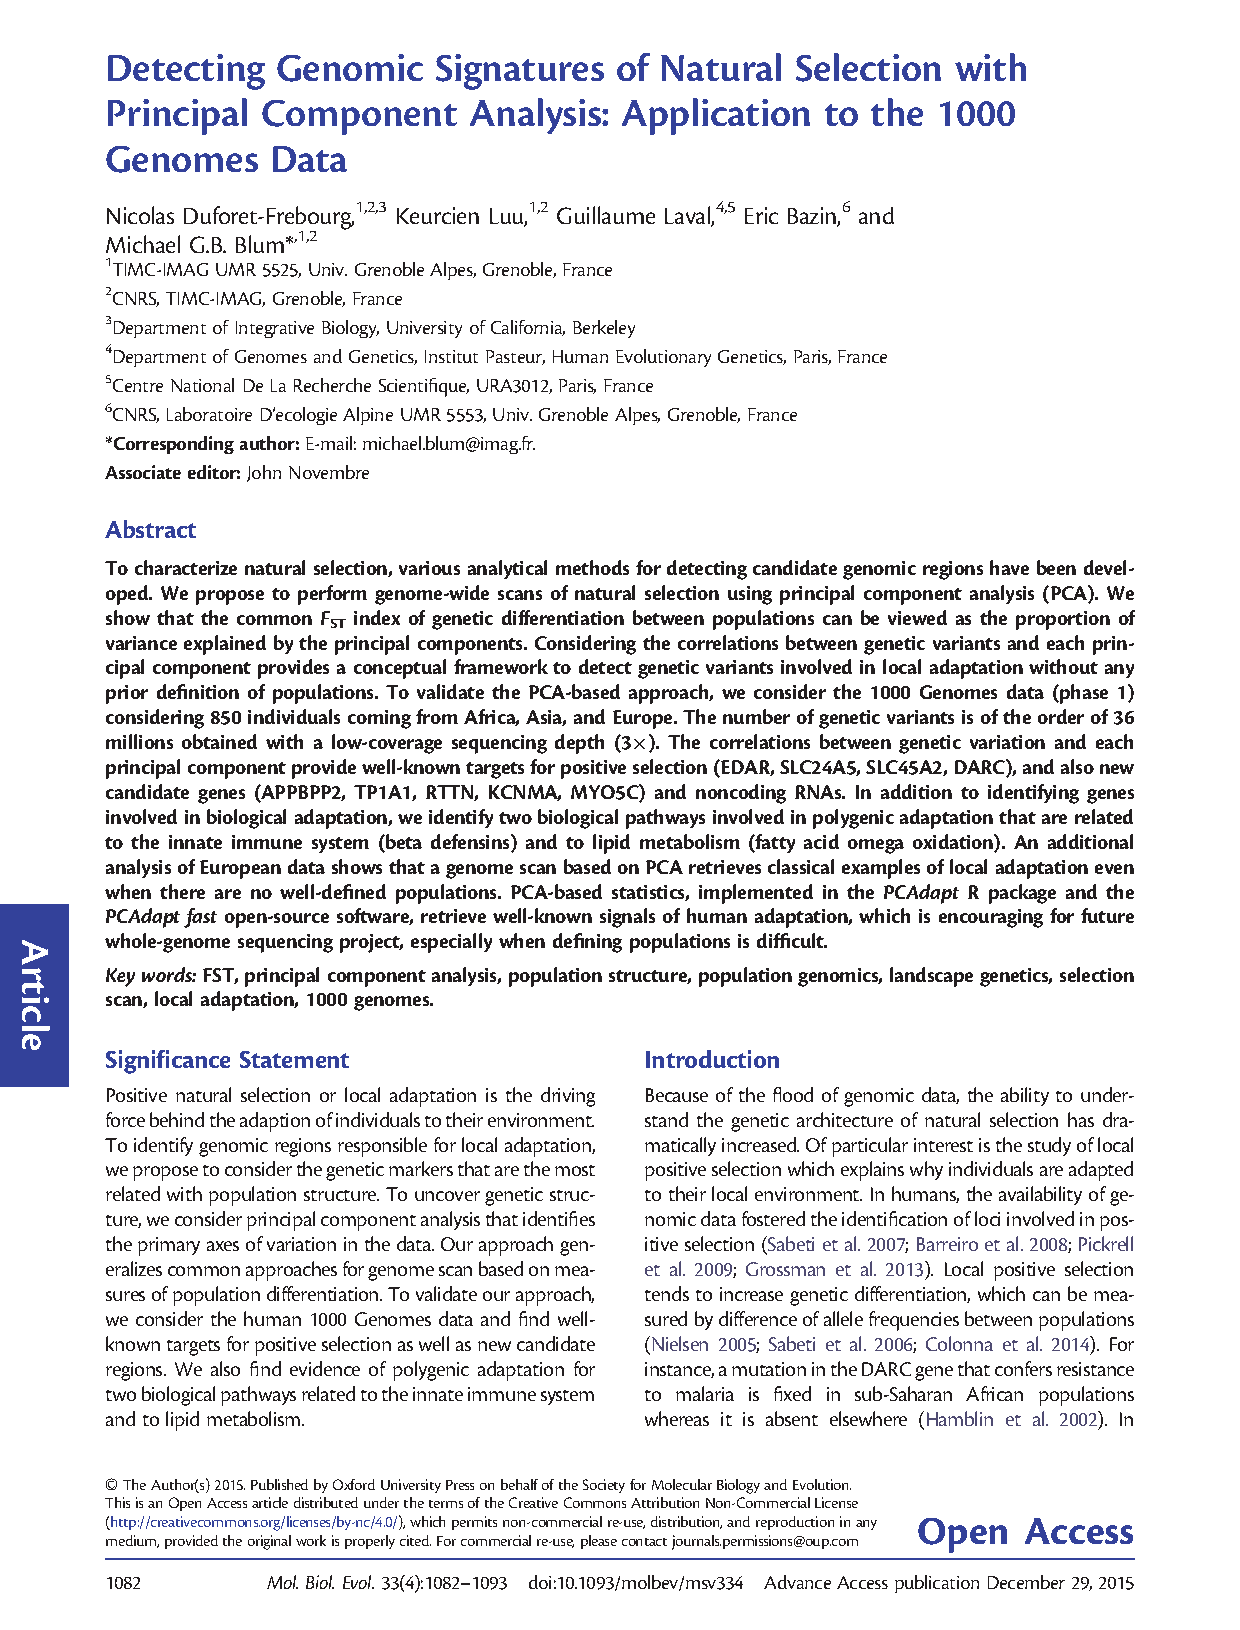
\includepdf[pages=-]{article/msv334.pdf}
  
  \newpage
  
  \section{La distance robuste de
  Mahalanobis}\label{la-distance-robuste-de-mahalanobis}
  
  \newpage
  
  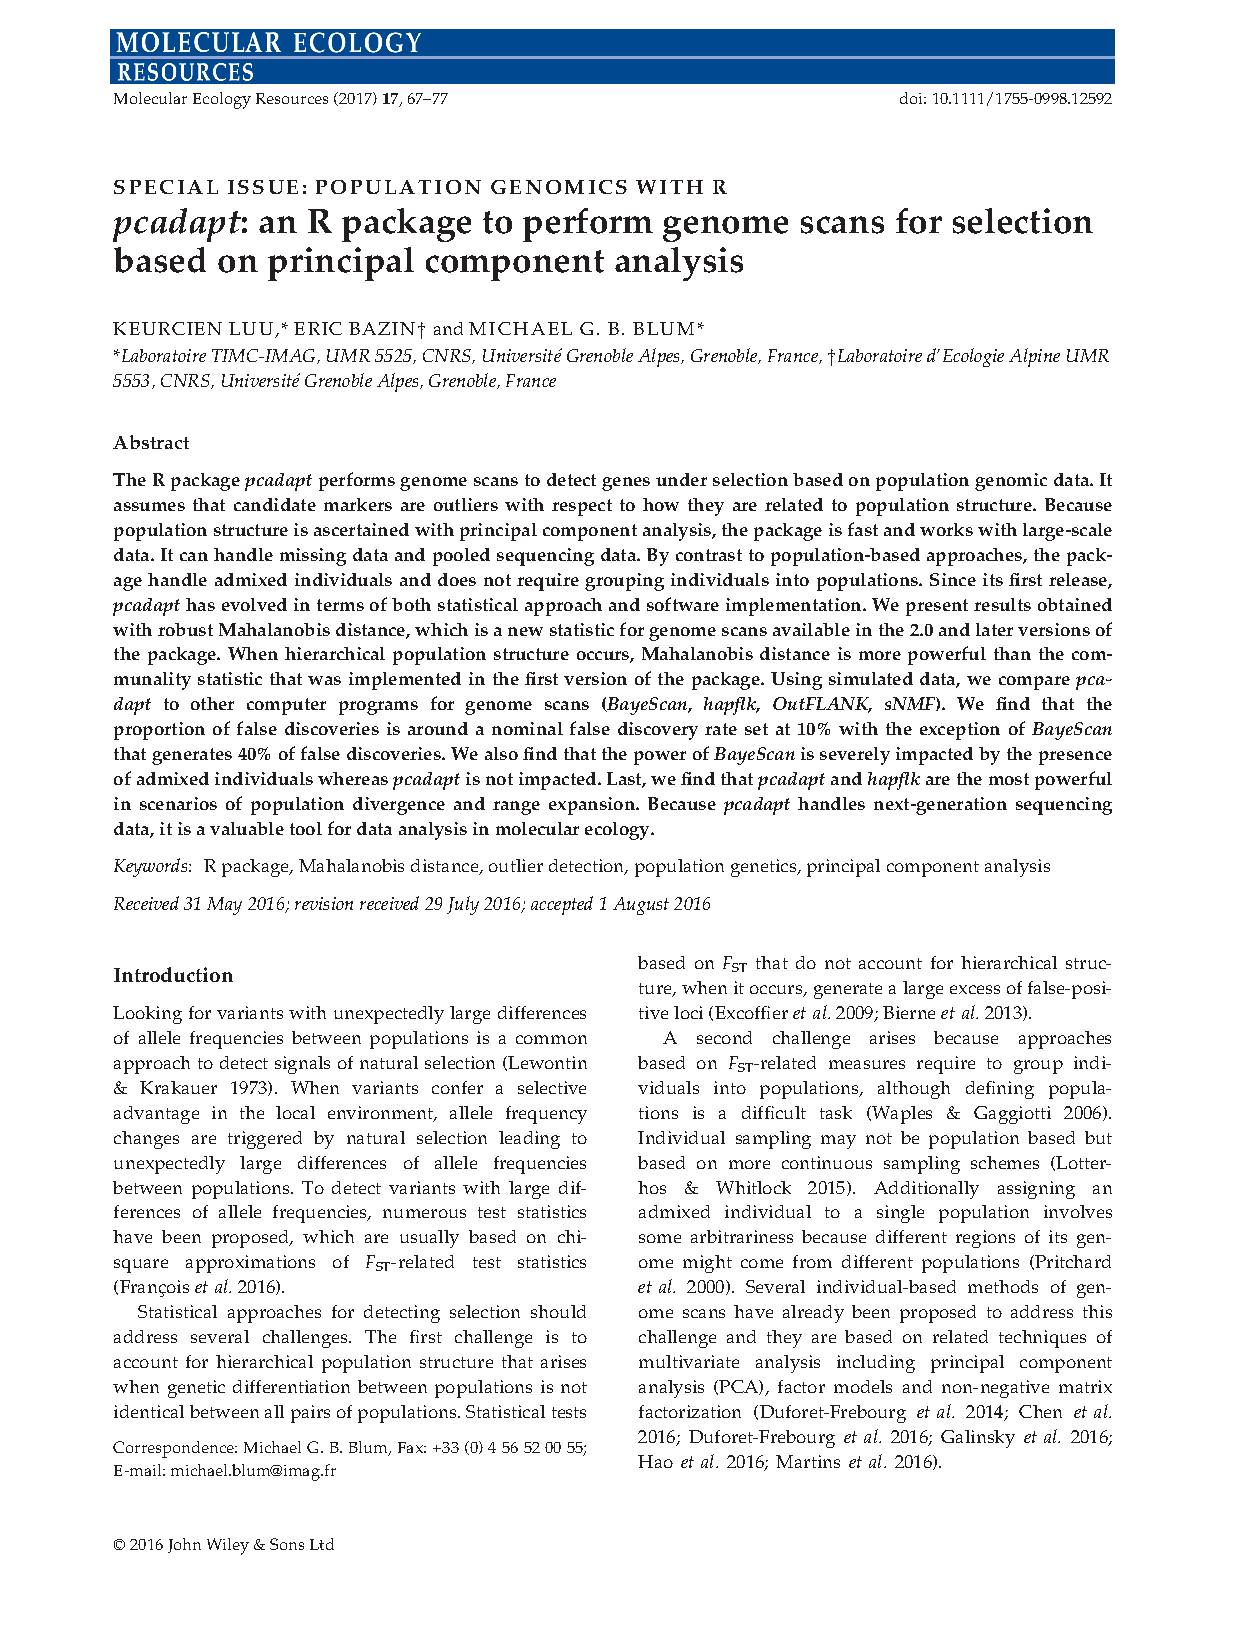
\includepdf[pages=-]{article/Luu_et_al-2017-Molecular_Ecology_Resources.pdf}
  
  \newpage
  
  \chapter{Introgression adaptative}\label{introgression-adaptative}
  
  \section{Qu'est-ce que l'introgression
  ?}\label{quest-ce-que-lintrogression}
  
  Avant de s'intéresser à la notion d'introgression, intéressons-nous
  d'abord à celle d'hybridation. L'hybridation peut être définie comme la
  reproduction entre deux individus appartenant à deux espèces ou à deux
  populations différentes. Cette définition nous amène à nous poser deux
  questions. La première, relative à la notion d'espèce, est souvent
  sujette à controverse. La seconde concerne quant à elle la désignation
  de populations différentes. Qu'est-ce qui fait que deux groupes
  d'individus sont différents ? Harrison suggère en 1990 que deux
  individus issus de populations différentes doivent chacun posséder des
  traits héritables qui les différencient (Harrison \& others, 1990).
  
  Nous parlons d'introgression lorsqu'un certain nombre de gènes est
  transféré d'une population à une autre.
  
  L'étude de régions génomiques présentant des caractéristiques
  d'introgression ou de divergence peut se révéler intéressante pour
  plusieurs raisons.
  
  \section{Coefficients de métissage globaux et
  locaux}\label{coefficients-de-metissage-globaux-et-locaux}
  
  Étant données des populations ancestrales, il est possible d'estimer
  pour un individu donné, la proportion de son génôme provenant de chacune
  des populations ancestrales. Ces proportions sont connues plus
  communément sous le nom de \emph{coefficients de métissage globaux}. De
  nombreux logiciels existent pour l'estimation de ces coefficients :
  STRUCTURE, ADMIXTURE (Alexander, Novembre, \& Lange, 2009), LEA (Frichot
  \& François, 2015), tess3r (Caye, Deist, Martins, Michel, \& François,
  2016). En complément à cette information globale, il peut être
  intéressant de déterminer sur des portions plus petites du génôme, de la
  même manière que dans le cas global, les proportions venant de telle ou
  telle population ancestrale pour chacune de ces portions. Nous parlons
  dans ce cas de \emph{coefficients de métissage locaux}. Encore une fois,
  plusieurs logiciels ont été proposés dans le but d'estimer ces
  coefficients : Hapmix (Price et al., 2009), EILA (Yang, Li, Buu, \&
  Williams, 2013), LAMP (Thornton \& Bermejo, 2014), loter ou encore RFmix
  (Maples, Gravel, Kenny, \& Bustamante, 2013).
  
  \section{Introgression}\label{introgression}
  
  L'introgression peut être détectée de différentes façons. Une première
  approche consiste à utiliser les \emph{coefficients de métissage
  locaux}. Les méthodes mentionnées plus haut estiment ces coefficients
  pour chaque individu, permettant de calculer à partir de ceux-ci des
  coefficients de métissage locaux pour chaque population.
  
  \section{Lien entre Analyse en Composantes Principales et métissage
  global.}\label{lien-entre-analyse-en-composantes-principales-et-metissage-global.}
  
  L'un des premiers articles à établir un lien entre l'ACP et les
  coefficients de métissage global fut sur l'interprétation généalogique
  de l'ACP de Gil McVean (McVean, 2009):
  
  \begin{figure}
  
  {\centering 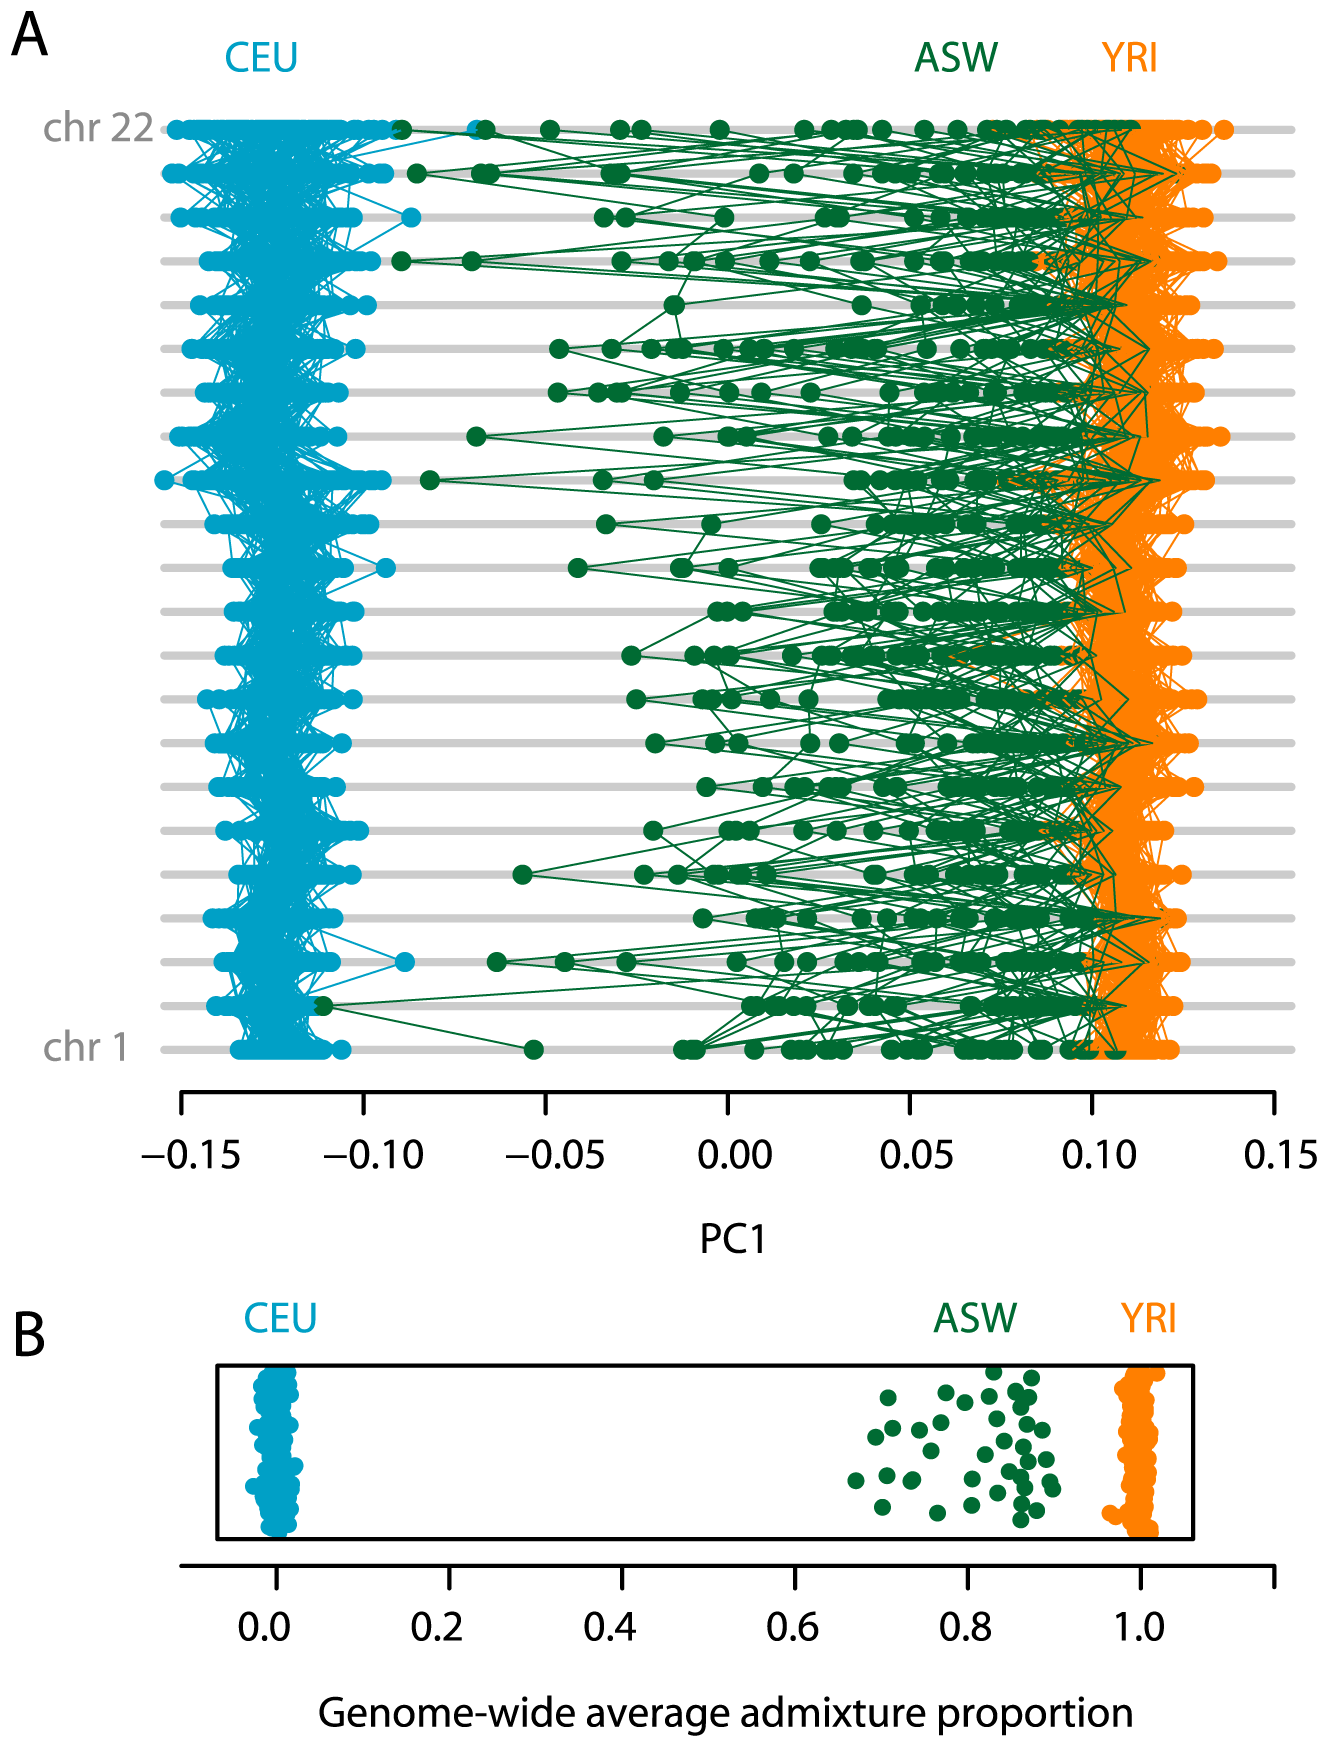
\includegraphics[width=300px]{figure/mcvean} 
  
  }
  
  \caption{Coefficients de métissage et ACP}\label{fig:mcvean}
  \end{figure}
  
  Pour chacun des 22 chromosomes,
  
  \section{Analyse en Composantes Principales
  locale}\label{analyse-en-composantes-principales-locale}
  
  Notant \(p\) le nombre de marqueurs génétiques, \(i\) un entier compris
  entre \(1\) et \(p\), et \(x_i\) la position génétique (en Morgans) ou
  la position physique (en paires de bases) du \(i\)-ème marqueur
  génétique. Nous définissons pour cet entier \(i\) la fenêtre \(W_i^T\)
  de taille \(T\) et centrée en \(i\) :
  
  \[W_i^T = \{ j \in [|1, p|], |x_i - x_j| \leq T/2 \}\]
  
  \section{Sensibilité à l'imputation des données
  manquantes}\label{sensibilite-a-limputation-des-donnees-manquantes}
  
  \newpage
  
  \subsection{Méthodes de détection}\label{methodes-de-detection}
  
  \subsubsection{Etat de l'art}\label{etat-de-lart-1}
  
  \paragraph{Scénario à flux de gènes}\label{scenario-a-flux-de-genes}
  
  \subparagraph{La statistique D de
  Patterson}\label{la-statistique-d-de-patterson}
  
  La statistique \(D\) de Patterson (Durand, Patterson, Reich, \& Slatkin,
  2011) demeure aujourd'hui la méthode la plus utilisée pour détecter la
  trace de flux de gènes dans une population. La méthode repose sur
  l'observation de motifs portant les noms \emph{ABBA} et \emph{BABA}, en
  référence aux différents types de généalogie possible pour un site
  nucléotidique.
  
  \[ D = \displaystyle \frac{\sum_i C_{ABBA}(i) - C_{BABA}(i)}{\sum_i C_{ABBA}(i) + C_{BABA}(i)} \]
  
  \subparagraph{RNDmin}\label{rndmin}
  
  {[}Descriptif de RNDmin{]}
  
  Pour comprendre la récente méthode proposée par (Rosenzweig, Pease,
  Besansky, \& Hahn, 2016), il est nécessaire de définir un certain nombre
  de statistiques dont \(RND_{\text{min}}\) dérive.
  
  ~
  
  \begin{itemize}
  \tightlist
  \item
    \(d_{xy}\) est la distance de Hamming entre la séquence \(X\) de la
    population \(1\) et la séquence \(Y\) de la population \(2\). Ainsi,
    si \(x = (x_i)_{1 \leq i \leq n}\) et \(y = (y_i)_{1 \leq i \leq n}\),
    alors :
  \end{itemize}
  
  \[d_{xy} = \text{Card}(\{i \in [|1, n|] \; | \; x_i \neq y_i \})\]
  
  Cette statistique est ainsi définie pour une paire de séquences (\(x\),
  \(y\)). Pour quantifier la dissimilarité entre deux ensembles de
  séquences, deux approches sont possibles. La première consiste à
  calculer la distance moyenne \(d_{XY}\). De par sa définition, cette
  distance présente néanmoins le défaut d'être peu sensible aux épisodes
  récents d'introgression (Geneva, Muirhead, Kingan, \& Garrigan, 2015).
  En effet, les faibles valeurs de \(d_{xy}\) correspondant à des
  évènements de divergence récents peuvent voir leur influence diminuée en
  cas de présence d'évènements de divergence plus anciens. Pour pallier à
  ce problème, considérer la distance minimale entre les deux ensembles de
  séquences (Joly, McLenachan, \& Lockhart, 2009) constitue une solution
  intéressante.
  
  {[}Expliquer pourquoi on définit \(d_{\text{out}}\) et \(RND\){]}
  
  En définissant \(d_{out} = \frac{1}{2}(d_{XO} + d_{YO})\), il est
  possible de définir de la même façon \(RND_{min}\) :
  
  \[RND_{\text{min}} = \frac{d_{\text{min}}}{d_{\text{out}}}\]
  
  Pour récapituler, \(RND_{\text{min}}\) est une statistique robuste aux
  variations de taux de mutation et qui reste sensible aux récents
  évènements d'introgression. En pratique, l'introduction de
  \(d_{\text{out}}\) requiert ainsi la donnée d'une population ancestrale
  commune aux deux populations d'intérêt.
  
  \subparagraph{Bdf}\label{bdf}
  
  \paragraph{Analyse Linéaire
  Discriminante}\label{analyse-lineaire-discriminante}
  
  \subsubsection{Régression linéaire, régression logistique, forêts
  aléatoires et importance des
  variables}\label{regression-lineaire-regression-logistique-forets-aleatoires-et-importance-des-variables}
  
  \subsubsection{Régression locale, package mgcv, locfit, Backward
  selection
  strategy}\label{regression-locale-package-mgcv-locfit-backward-selection-strategy}
  
  \subsubsection{ACP locale et espace de
  formes}\label{acp-locale-et-espace-de-formes}
  
  \newpage
  
  \section{Simulations}\label{simulations}
  
  \subsection{Données de peupliers}\label{donnees-de-peupliers}
  
  Le premier jeu de données est issu d'une étude d'introgression
  adaptative chez les peupliers d'Amérique du Nord (Suarez-Gonzalez,
  2016). La simulation d'haplotypes d'individus admixés est effectuée à
  partir des deux populations ancestrales qui y sont présentes. La
  première, \emph{Populus Balsamifera}, est une espèce de peupliers qui
  peuple le nord du continent nord-américain, d'Est en Ouest, et se trouve
  exposée à des conditions climatiques peu clémentes.La seconde,
  \emph{Populus Trichocarpa}, est principalement localisée en Californie,
  et bénéficie d'un climat continental.
  
  Chacune des simulations est constituée de \(50\) haplotypes de la souche
  continentale, de \(50\) haplotyêpes de la souche boréale, ainsi que de
  \(50\) haplotypes d'individus hybrides générés à partir des haplotypes
  ancestraux. Ces haplotypes ancestraux ont été estimés à l'aide du
  logiciel Beagle. A partir des positions en paires de base, une carte de
  recombinaison génétique est générée en utilisant le taux de
  recombinaison moyen chez le peuplier. Le taux de recombinaison, noté
  \(\tau_r\), correspond au nombre moyen de paires de bases à parcourir
  pour qu'ait lieu un épisode de recombinaison génétique, \emph{i.e.},
  notant \(L\) la longueur du chromosome en Morgans (\(M\)), et \(N_{bp}\)
  le nombre de paires de bases le constituant, le taux de recombinaison
  génétique pour ce chromosome est donné par la relation:
  
  \[\tau_r = \frac{L}{N_{bp}}\]
  
  Dans ce scénario, les simulations ont été produites en utilisant un taux
  de recombinaison génétique moyen \(\tau_r\) de \(0.05\) centiMorgans par
  million de paire de bases, correspondant à la valeur utilisée par les
  auteurs de l'étude avec le logiciel RASPberry
  (\textit{Recombination via Ancestry Switch Probability}). A partir de la
  donnée de la position physique en paires de bases ainsi que du taux de
  recombinaison moyen, nous générons une carte de recombinaison génétique
  adaptée à nos simulations.
  
  \subsection{Génération aléatoire d'individus
  hybrides}\label{generation-aleatoire-dindividus-hybrides}
  
  Pour simuler un individu métissé, il est d'abord nécessaire de simuler
  l'emplacement des évènements de recombinaison. Pour ce faire, nous
  utilisons le modèle décrit dans (Price et al., 2009), en parcourant
  
  \begin{figure}
  
  {\centering 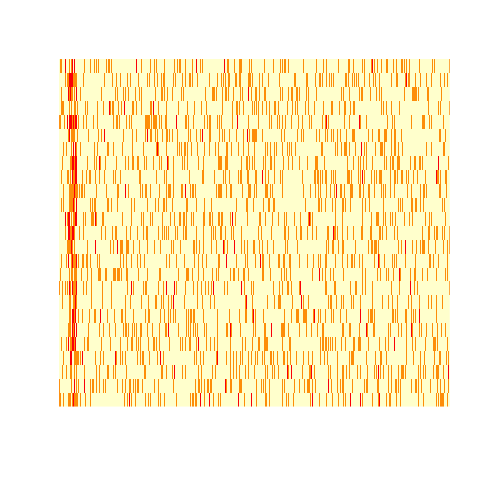
\includegraphics[width=400px,height=200px]{figure/ancestry_heatmap_lambda_0001} 
  
  }
  
  \caption{$\lambda = 0.001$}\label{fig:lambda0001}
  \end{figure}\begin{figure}
  
  {\centering 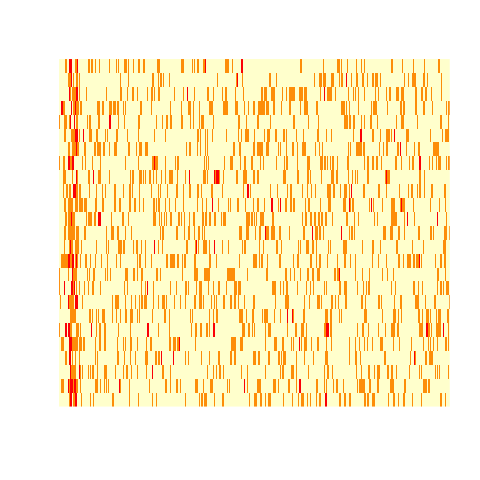
\includegraphics[width=400px,height=200px]{figure/ancestry_heatmap_lambda_001} 
  
  }
  
  \caption{$\lambda = 0.01$}\label{fig:lambda001}
  \end{figure}\begin{figure}
  
  {\centering 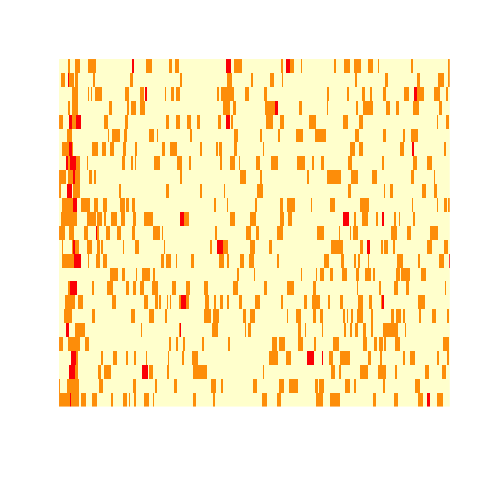
\includegraphics[width=400px,height=200px]{figure/ancestry_heatmap_lambda_01} 
  
  }
  
  \caption{$\lambda = 0.1$}\label{fig:lambda01}
  \end{figure}
  
  \newpage
  
  \subsection{Simulations à partir de ms et
  Seq-Gen}\label{simulations-a-partir-de-ms-et-seq-gen}
  
  Dans le scénario d'introgression via flux de gènes, nous nous inspirons
  des modèles de simulation décrits dans (Martin \& Jiggins, 2015). Ces
  modèles sont largement repris dans la littérature pour l'évaluation de
  statistiques telles que \(RND_{min}\) (Rosenzweig et al., 2016) et
  \(Bd_f\) (Pfeifer \& Kapan, 2017). Chaque simulation est constituée de
  100 individus. Un individu est généré en concaténant un certain nombre
  de séquences de nucléotides, d'une longueur fixée à 5000 paires de bases
  par séquence. Chacune de ces séquences est elle-même simulée suivant un
  modèle neutre ou alternatif. Le modèle neutre décrit un scénario
  démographique classique de populations divergentes. Le modèle alternatif
  décrit quant à lui un scénario légèrement différent, et servira à
  caractériser les séquences \emph{introgressées}. Les lignes de commande
  \emph{ms} permettant de générer les séquences de nucléotides pour le
  modèle neutre ainsi que pour le modèle alternatif sont données
  ci-dessous :
  
  ~
  
  \begin{itemize}
  \tightlist
  \item
    Modèle neutre :
  \end{itemize}
  
  \begin{verbatim}
  ./ms 200 1 -I 4 50 50 50 50 -ej 1 2 1 -ej 2 3 1 -ej 3 4 1 
  -r 50 5000 -T 
  \end{verbatim}
  
  \begin{figure}
  
  {\centering 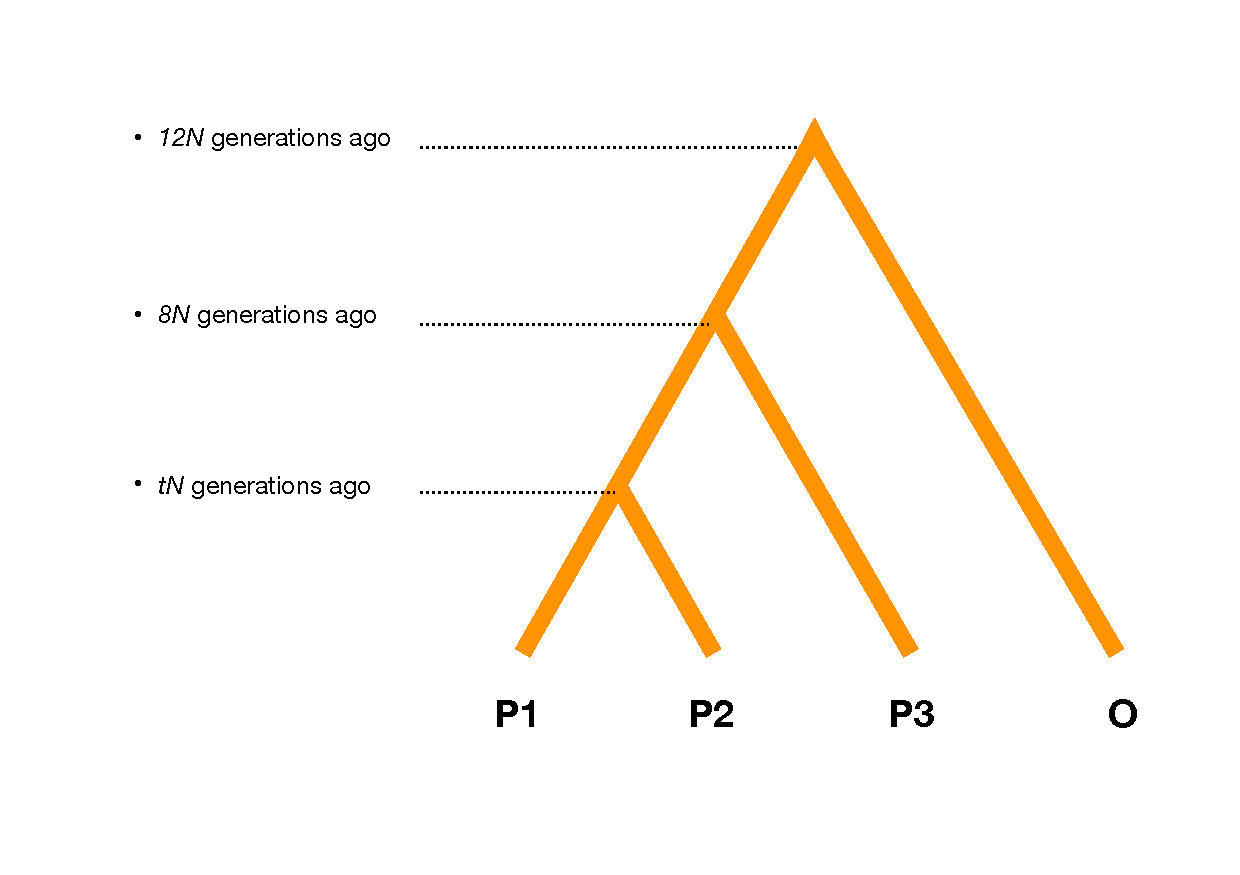
\includegraphics[scale=0.5]{figure/background} 
  
  }
  
  \caption{Modèle neutre. $12N$ genérations auparavant, premier épisode de divergence donnant naissance à P1 et à O. $8N$ générations auparavant, deuxième épisode de divergence voyant l'apparition de P3. $4N$ générations auparavant, dernier épisode de divergence et apparition de P2.}\label{fig:background}
  \end{figure}
  
  ~
  
  \begin{itemize}
  \tightlist
  \item
    Modèle alternatif :
  \end{itemize}
  
  \begin{verbatim}
  ./ms 200 1 -I 4 50 50 50 50 -ej 1 2 1 -ej 2 3 1 -ej 3 4 1 
  -es 0.1 2 0.8 -ej 0.1 5 3 -r 50 5000 -T
  \end{verbatim}
  
  \begin{figure}
  
  {\centering 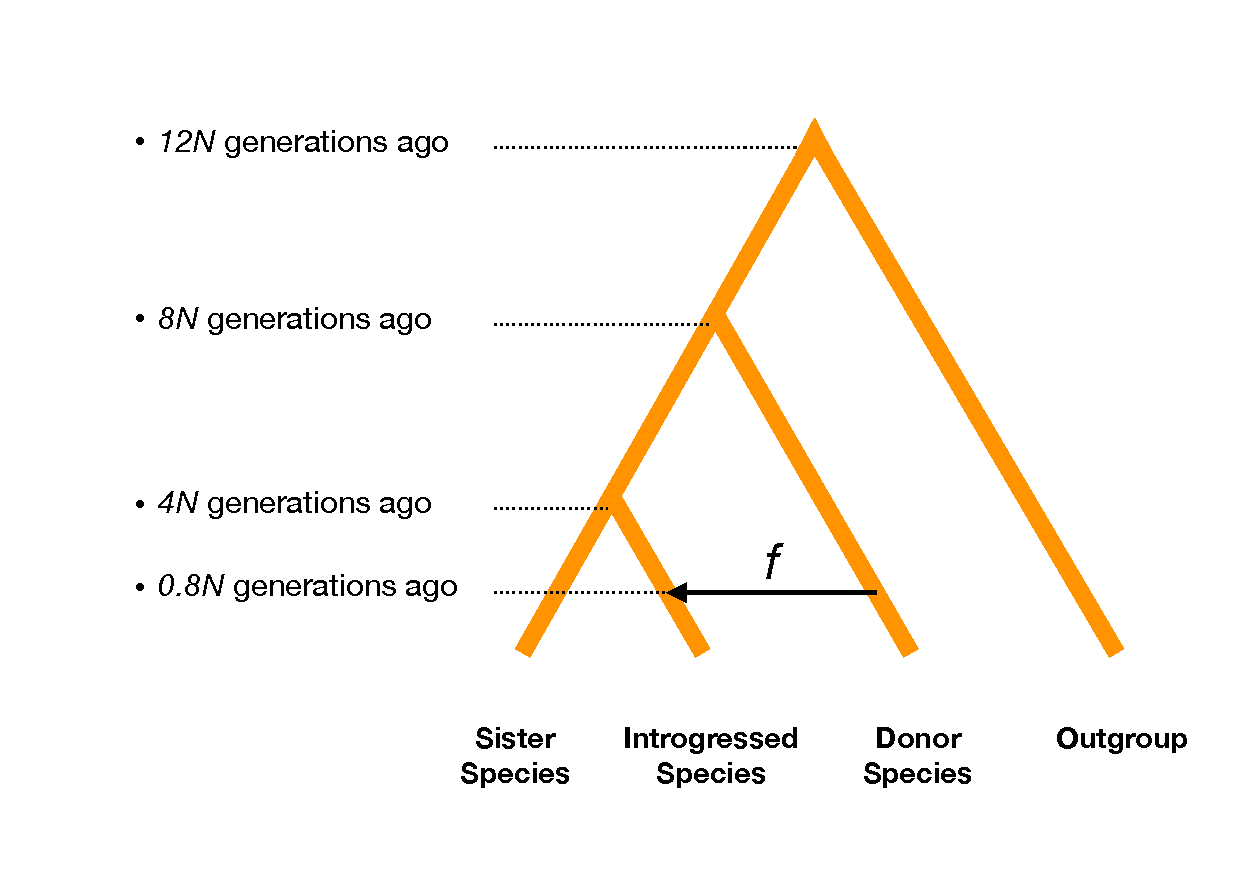
\includegraphics[scale=0.5]{figure/alternate} 
  
  }
  
  \caption{Modèle alternatif. $12N$ genérations auparavant, premier épisode de divergence donnant naissance à P1 et à O. $8N$ générations auparavant, deuxième épisode de divergence voyant l'apparition de P3. $4N$ générations auparavant, dernier épisode de divergence et apparition de P2. $t$ unités de temps auparavant, épisode de flux de gènes de P3 vers la population P2.}\label{fig:alternate}
  \end{figure}
  
  La variable \(f\) présente en figure \ref{fig:alternate} représente le
  taux d'introgression, elle quantifie la proportion d'haplotypes présents
  dans la population P2 et qui proviennent de la population P3. Ainsi, une
  valeur de \(f\) égale à \(1\) reviendrait à simuler un épisode de
  divergence de la population P3, duquel découlerait la naissance de la
  population P2. La valeur de \(f\) utilisée ci-dessus est \(0.2\),
  signifiant que 20\% des haplotypes présents dans la population 2 sont
  issus de la population P3.
  
  \subsection{Résultats de la comparaison des
  logiciels}\label{resultats-de-la-comparaison-des-logiciels}
  
  \begin{Shaded}
  \begin{Highlighting}[]
  \NormalTok{im.df <-}\StringTok{ }\KeywordTok{data.frame}\NormalTok{(}\DataTypeTok{methods =} \KeywordTok{c}\NormalTok{(}\StringTok{"Bdf"}\NormalTok{, }\StringTok{"D"}\NormalTok{, }\StringTok{"f_d"}\NormalTok{, }\StringTok{"pcadapt"}\NormalTok{, }\StringTok{"RNDmin"}\NormalTok{),}
                      \DataTypeTok{input =} \KeywordTok{c}\NormalTok{(}\StringTok{"genoytpes"}\NormalTok{, }\StringTok{"genoytpes"}\NormalTok{, }\StringTok{"genoytpes"}\NormalTok{, }\StringTok{"genoytpes"}\NormalTok{, }\StringTok{"haplotypes"}\NormalTok{),}
                      \DataTypeTok{nb_of_pop =} \KeywordTok{c}\NormalTok{(}\StringTok{"4"}\NormalTok{, }\StringTok{"4"}\NormalTok{, }\StringTok{"4"}\NormalTok{, }\StringTok{">= 3"}\NormalTok{, }\StringTok{"3"}\NormalTok{),}
                      \DataTypeTok{outgroup =} \KeywordTok{c}\NormalTok{(}\StringTok{"Oui"}\NormalTok{, }\StringTok{"Oui"}\NormalTok{, }\StringTok{"Oui"}\NormalTok{, }\StringTok{"Oui"}\NormalTok{, }\StringTok{"Oui"}\NormalTok{))}
  
  \NormalTok{knitr::}\KeywordTok{kable}\NormalTok{(im.df, }
               \DataTypeTok{col.names =} \KeywordTok{c}\NormalTok{(}\StringTok{"Statistique"}\NormalTok{, }
                             \StringTok{"Format"}\NormalTok{,}
                             \StringTok{"Nombre de populations"}\NormalTok{, }
                             \StringTok{"Dont Outgroup"}\NormalTok{), }
               \DataTypeTok{format =} \StringTok{"latex"}\NormalTok{)}
  \end{Highlighting}
  \end{Shaded}
  
  \begin{tabular}{l|l|l|l}
  \hline
  Statistique & Format & Nombre de populations & Dont Outgroup\\
  \hline
  Bdf & genoytpes & 4 & Oui\\
  \hline
  D & genoytpes & 4 & Oui\\
  \hline
  f\_d & genoytpes & 4 & Oui\\
  \hline
  pcadapt & genoytpes & >= 3 & Oui\\
  \hline
  RNDmin & haplotypes & 3 & Oui\\
  \hline
  \end{tabular}
  
  \paragraph{Scénario de métissage}\label{scenario-de-metissage}
  
  Nous comparons ici notre méthode au logiciel RFMix destiné à la
  détermination de coefficients de métissage local.
  
  \begin{figure}
  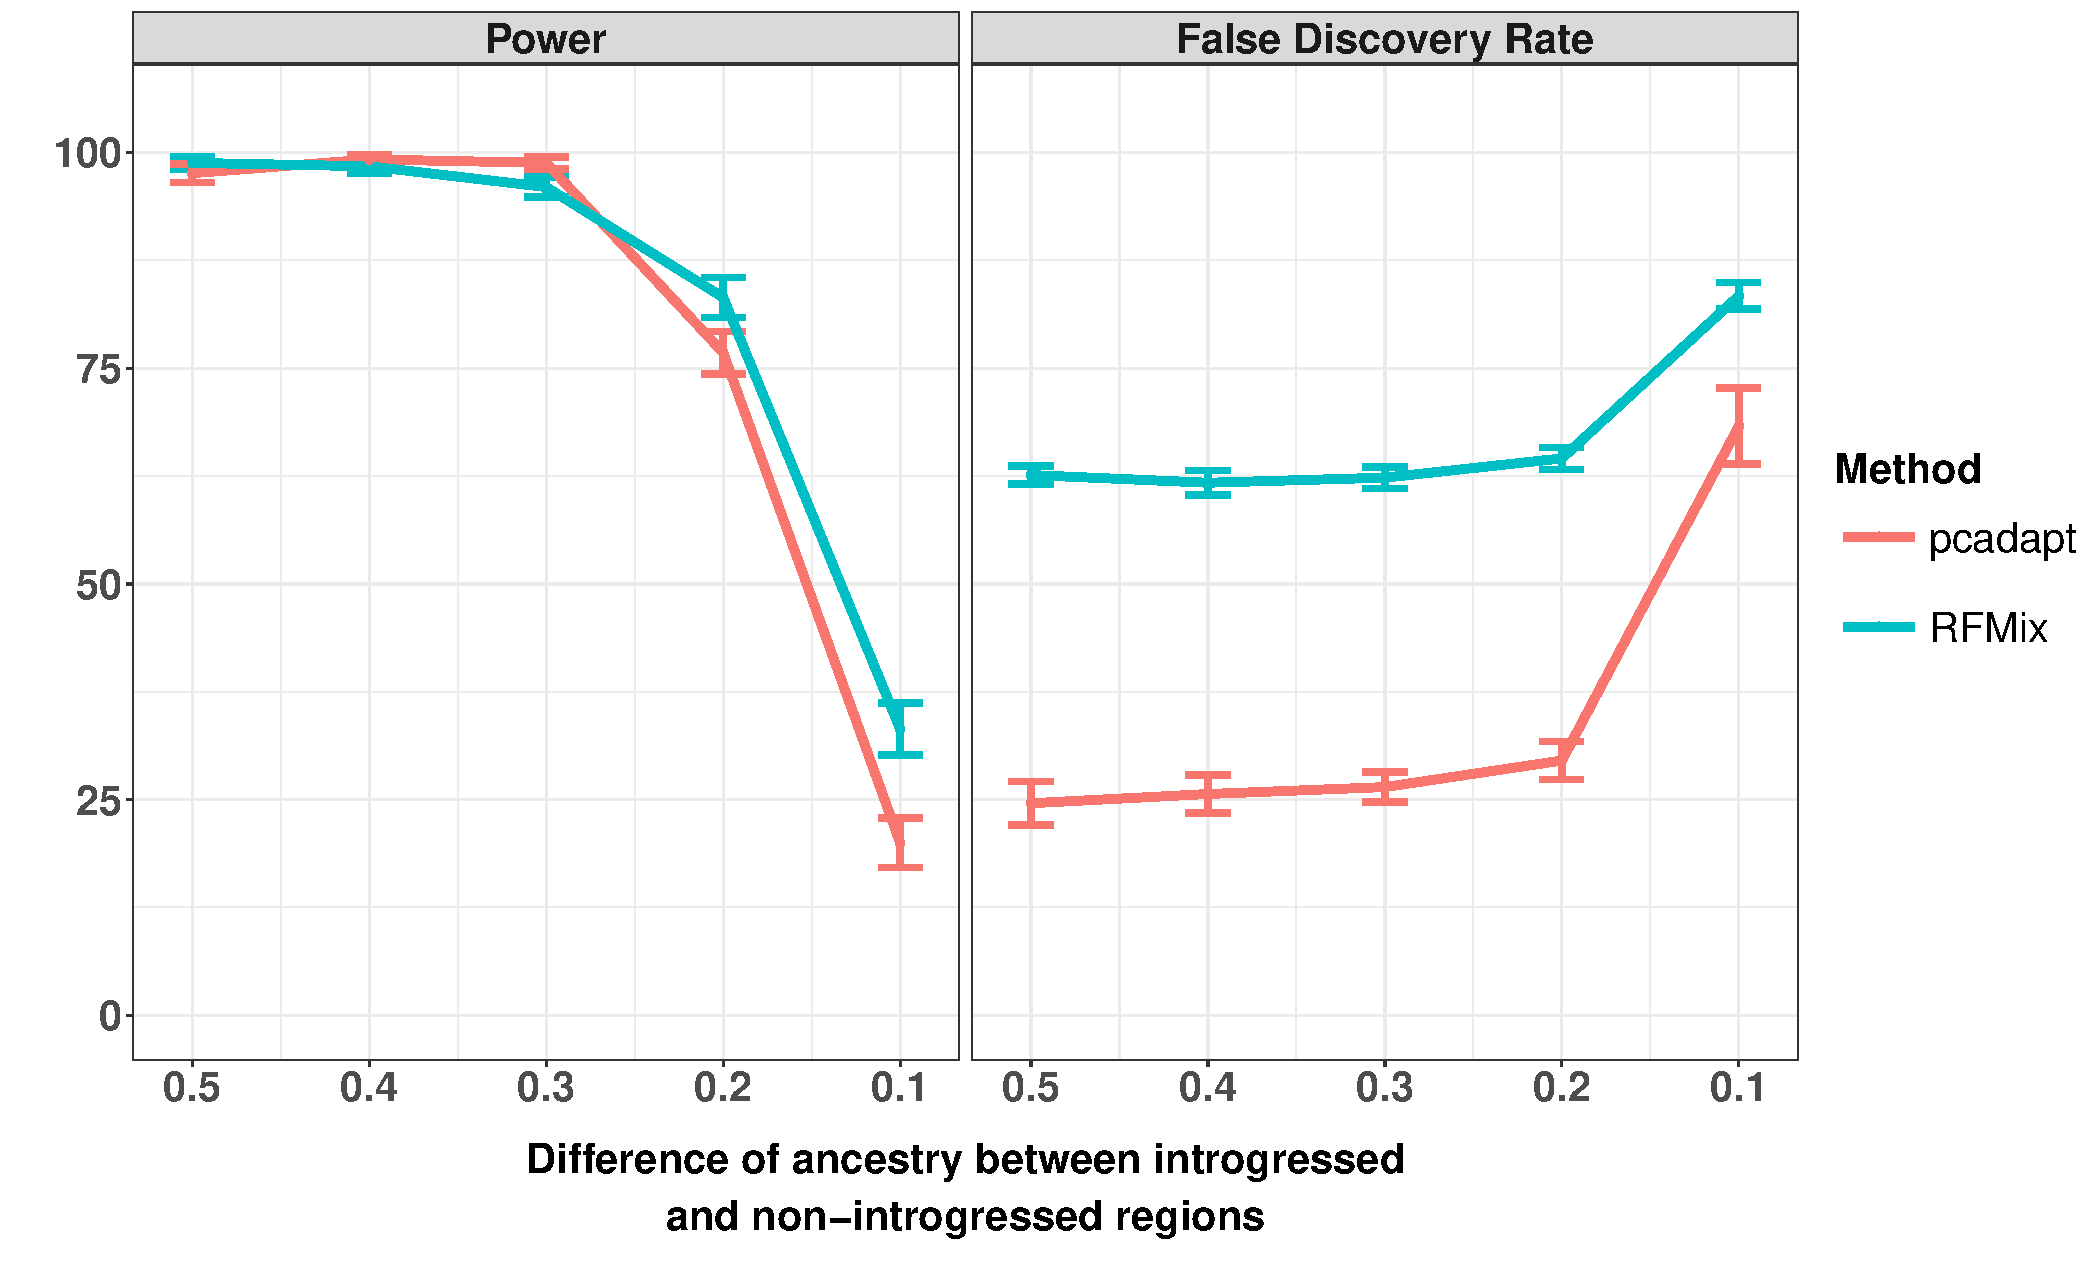
\includegraphics[width=500px]{figure/facet_admixture_setting_10_gen} \caption{10 generations}\label{fig:ras10g}
  \end{figure}
  
  \begin{figure}
  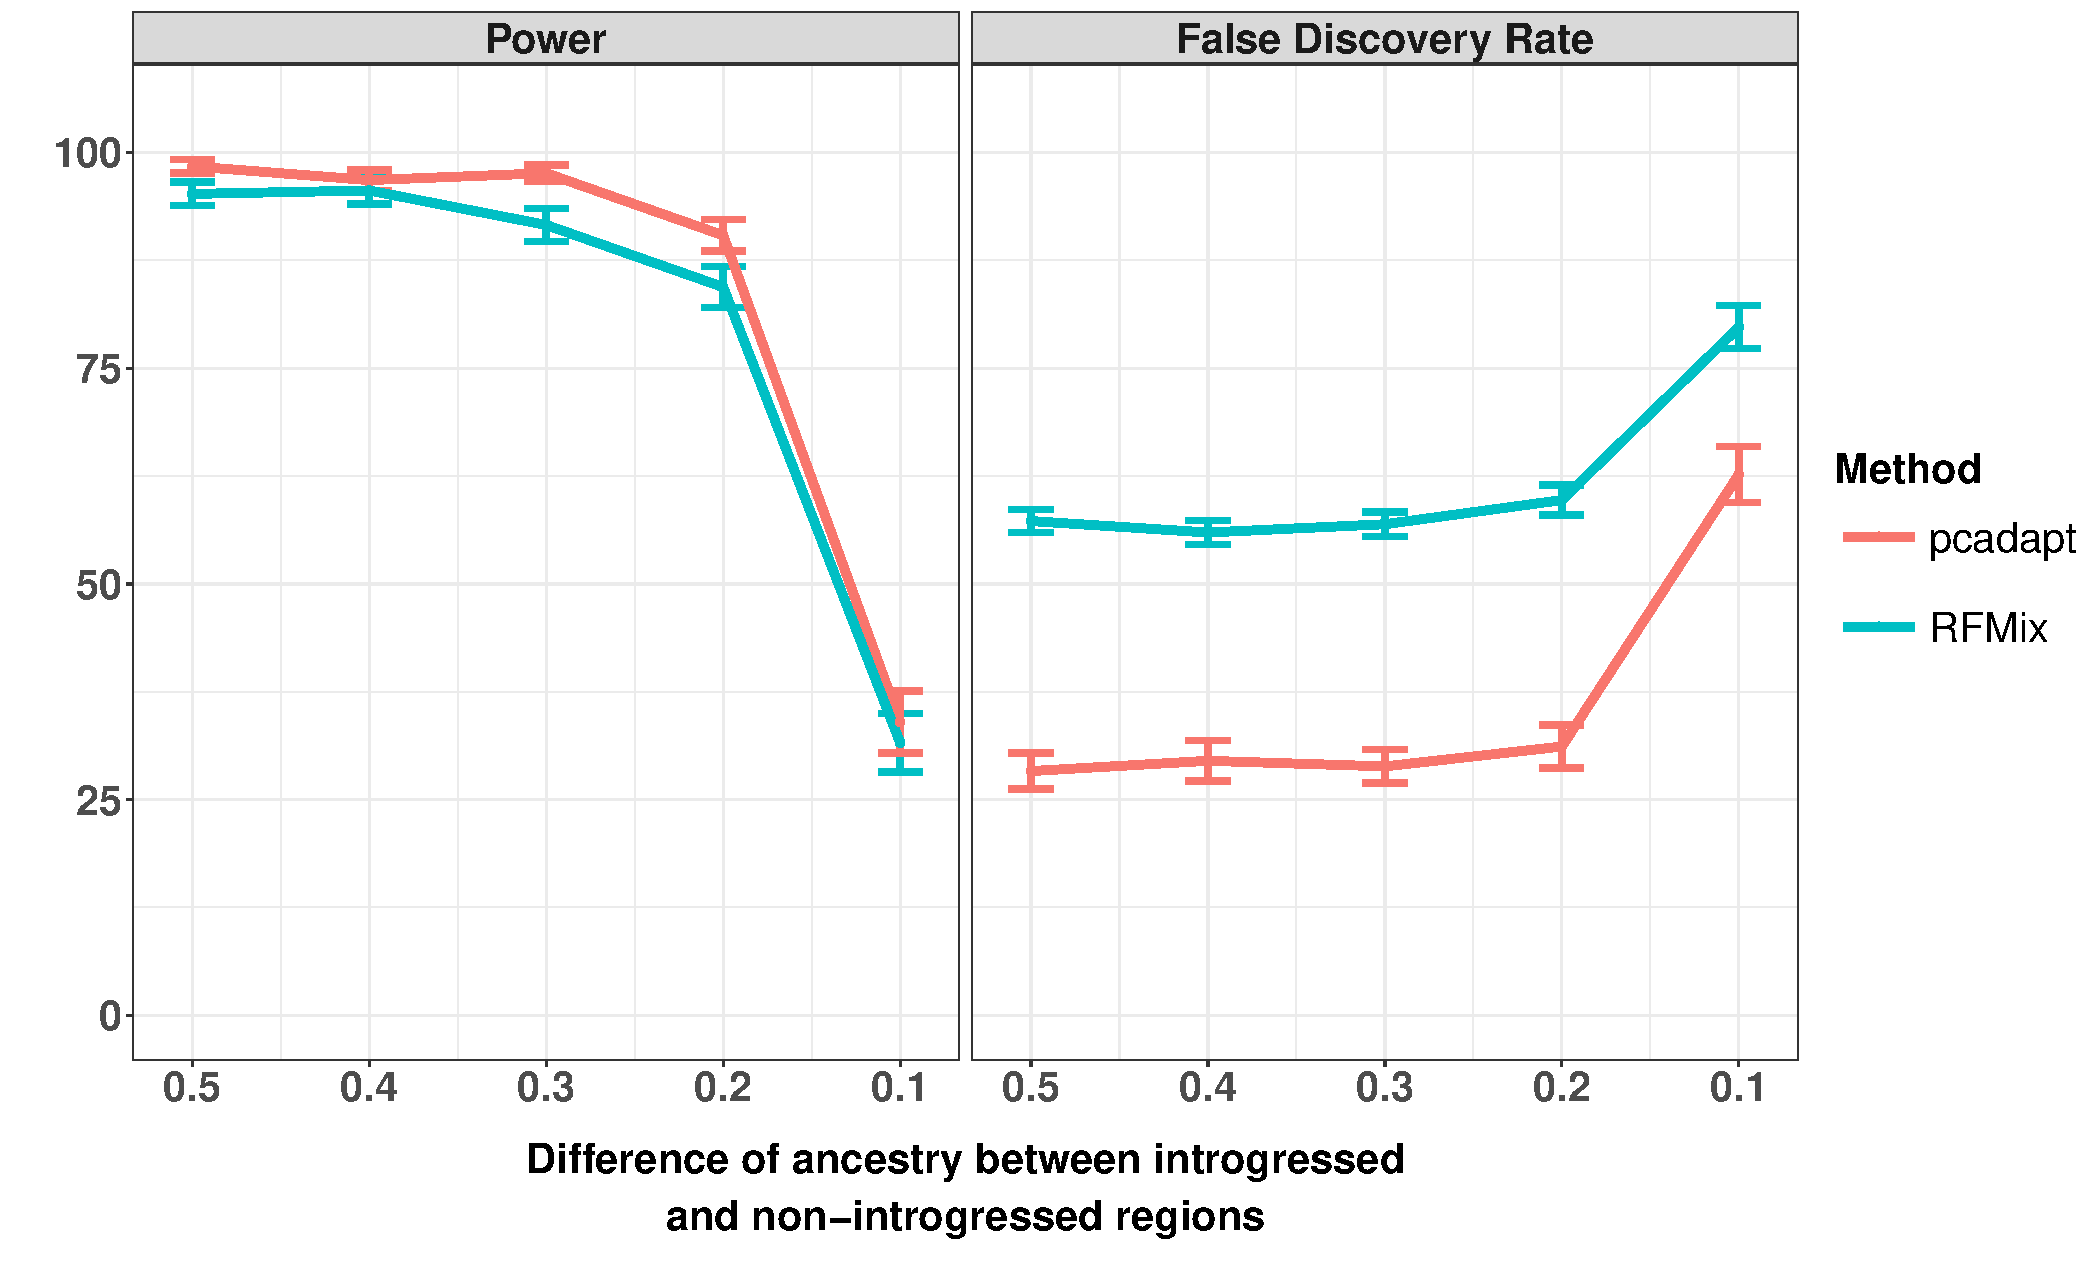
\includegraphics[width=500px]{figure/facet_admixture_setting_100_gen} \caption{100 generations}\label{fig:ras100g}
  \end{figure}
  
  \begin{figure}
  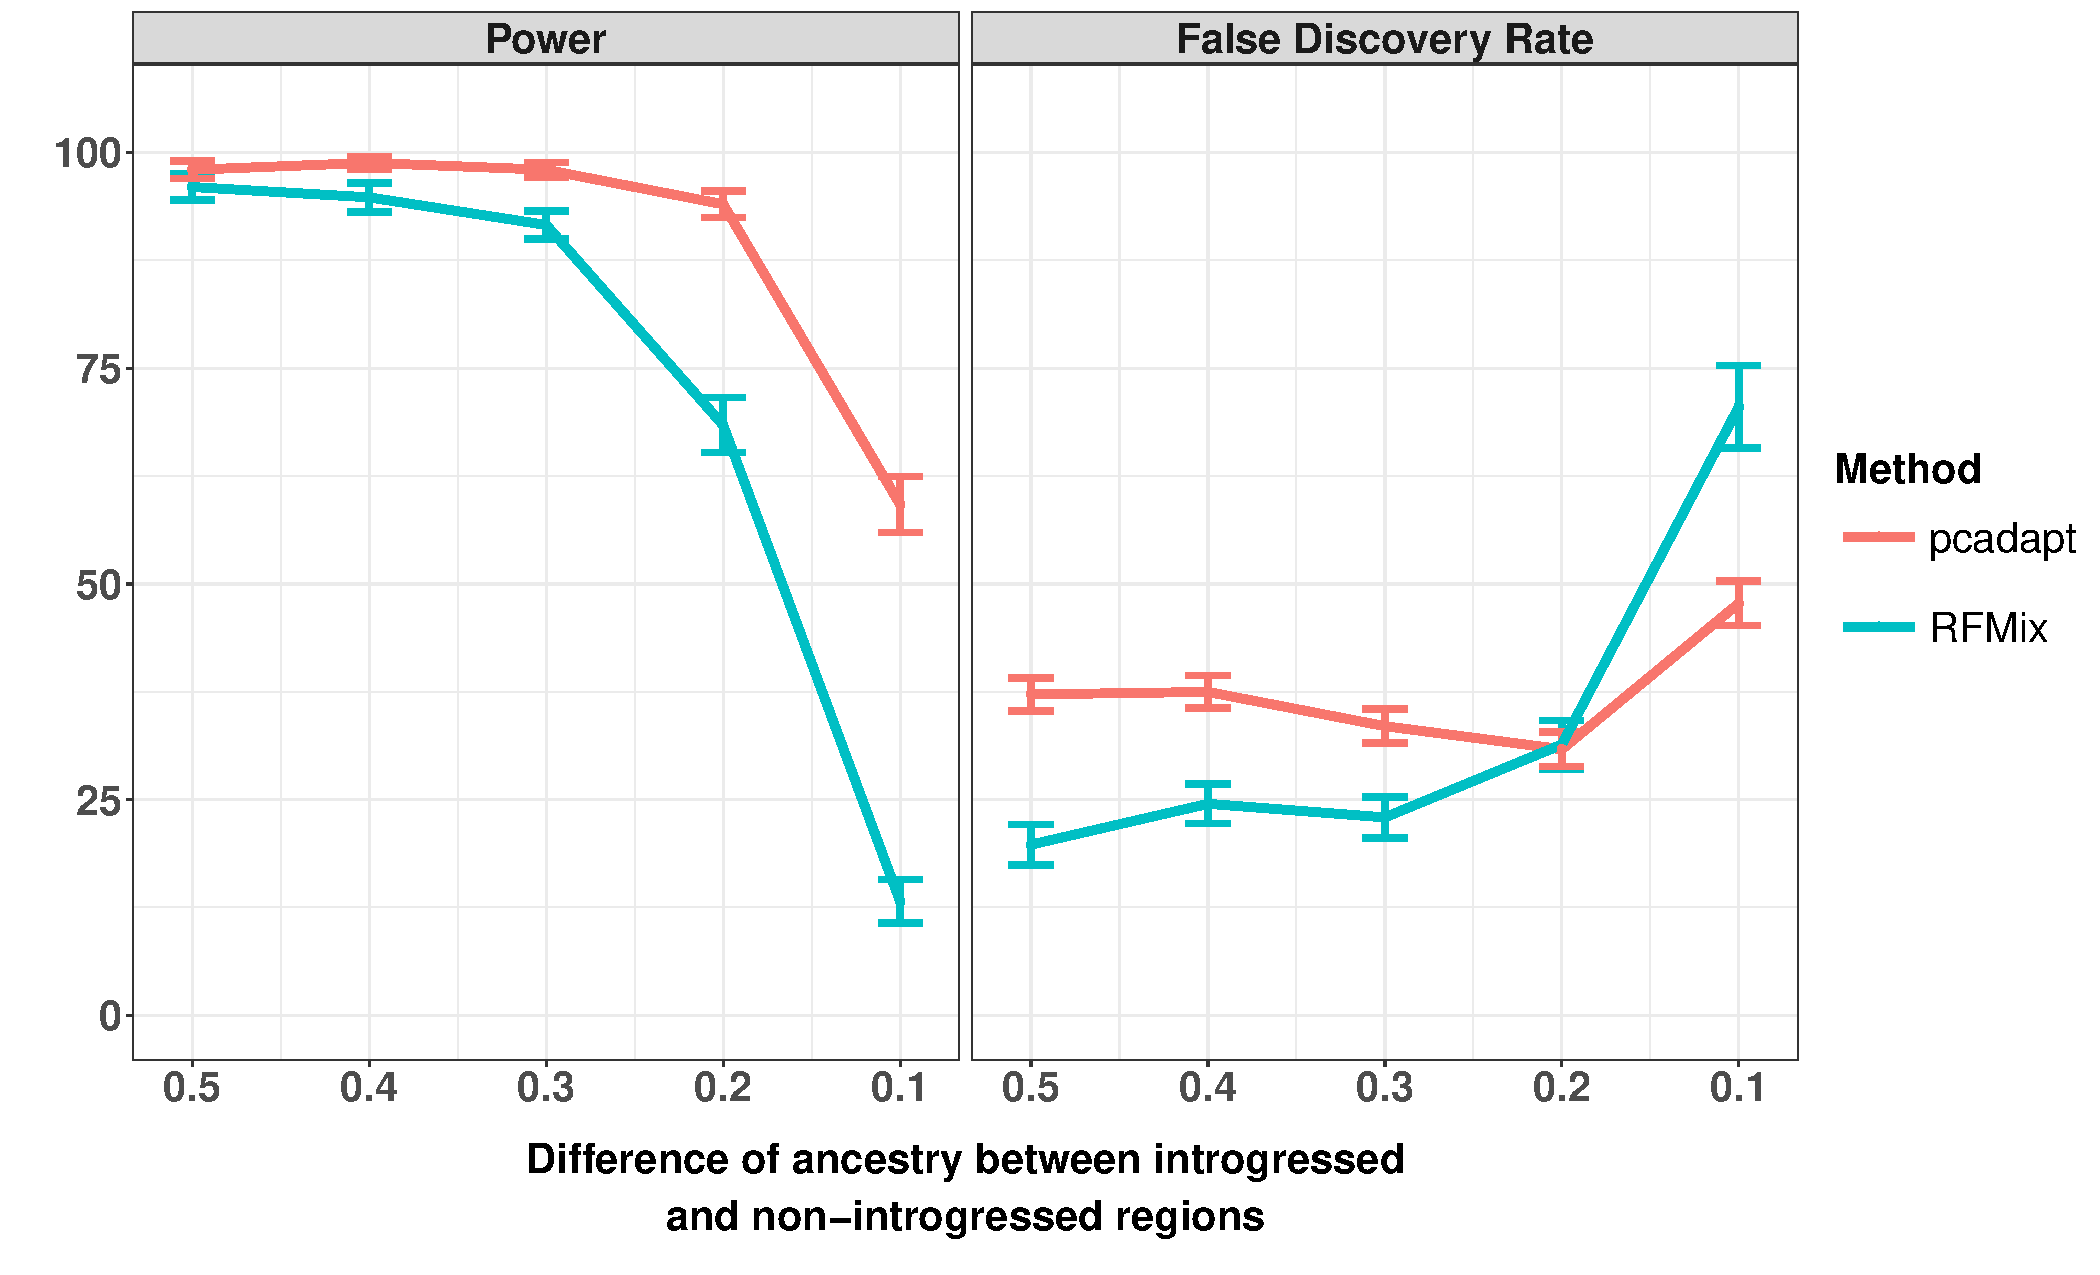
\includegraphics[width=500px]{figure/facet_admixture_setting_1000_gen} \caption{1000 generations}\label{fig:ras1000g}
  \end{figure}
  
  \paragraph{Scénario à flux de gènes}\label{scenario-a-flux-de-genes-1}
  
  Dans ce paragraphe, nous comparons notre statistique de test à un
  ensemble de statistiques implémentées dans le package R \emph{PopGenome}
  : la statistique \(D\) de Patterson, RNDmin (Rosenzweig et al., 2016) et
  BDF (Pfeifer \& Kapan, 2017).
  
  \chapter{Aspect computationnel}\label{aspect-computationnel}
  
  Dans cette partie, nous nous intéresserons brièvement à l'aspect
  computationnel des méthodes qui ont été présentées dans les chapitres
  précédents. Le développement d'outils logiciels destinés à l'exploration
  de données génétiques volumineuses requiert qu'une attention toute
  particulière soit portée à l'utilisation des ressources de calcul.
  
  Blockwise computation of covariance matrix Random SVD Storage in binary
  format Memory-mapping
  
  \chapter*{Conclusion}\label{conclusion}
  \addcontentsline{toc}{chapter}{Conclusion}
  
  If we don't want Conclusion to have a chapter number next to it, we can
  add the \texttt{\{-\}} attribute.
  
  \textbf{More info}
  
  And here's some other random info: the first paragraph after a chapter
  title or section head \emph{shouldn't be} indented, because indents are
  to tell the reader that you're starting a new paragraph. Since that's
  obvious after a chapter or section title, proper typesetting doesn't add
  an indent there.
  
  \appendix
  
  \chapter{The First Appendix}\label{the-first-appendix}
  
  This first appendix includes all of the R chunks of code that were
  hidden throughout the document (using the \texttt{include\ =\ FALSE}
  chunk tag) to help with readibility and/or setup.
  
  \textbf{In the main Rmd file}
  
  \begin{Shaded}
  \begin{Highlighting}[]
  \CommentTok{# This chunk ensures that the thesisdown package is}
  \CommentTok{# installed and loaded. This thesisdown package includes}
  \CommentTok{# the template files for the thesis and also two functions}
  \CommentTok{# used for labeling and referencing}
  \CommentTok{#opts_chunk$set(cache=TRUE)}
  
  \NormalTok{if(!}\KeywordTok{require}\NormalTok{(devtools))\{}
    \KeywordTok{install.packages}\NormalTok{(}\StringTok{"devtools"}\NormalTok{, }\DataTypeTok{repos =} \StringTok{"http://cran.rstudio.com"}\NormalTok{)}
  \NormalTok{\}}
  
  \NormalTok{if(!}\KeywordTok{require}\NormalTok{(dplyr))\{}
    \KeywordTok{install.packages}\NormalTok{(}\StringTok{"dplyr"}\NormalTok{, }\DataTypeTok{repos =} \StringTok{"http://cran.rstudio.com"}\NormalTok{)}
  \NormalTok{\}}
  
  \NormalTok{if(!}\KeywordTok{require}\NormalTok{(ggplot2))\{}
    \KeywordTok{install.packages}\NormalTok{(}\StringTok{"ggplot2"}\NormalTok{, }\DataTypeTok{repos =} \StringTok{"http://cran.rstudio.com"}\NormalTok{)}
  \NormalTok{\}}
  
  \NormalTok{if(!}\KeywordTok{require}\NormalTok{(bookdown))\{}
    \KeywordTok{install.packages}\NormalTok{(}\StringTok{"bookdown"}\NormalTok{, }\DataTypeTok{repos =} \StringTok{"http://cran.rstudio.com"}\NormalTok{)}
  \NormalTok{\}}
  
  \NormalTok{if(!}\KeywordTok{require}\NormalTok{(thesisdown))\{}
    \KeywordTok{library}\NormalTok{(devtools)}
    \NormalTok{devtools::}\KeywordTok{install_github}\NormalTok{(}\StringTok{"ismayc/thesisdown"}\NormalTok{)}
  \NormalTok{\}}
  
  \NormalTok{if(!}\KeywordTok{require}\NormalTok{(data.table))\{}
    \KeywordTok{install.packages}\NormalTok{(}\StringTok{"data.table"}\NormalTok{, }\DataTypeTok{repos =} \StringTok{"http://cran.rstudio.com"}\NormalTok{)}
  \NormalTok{\}}
  
  \NormalTok{if(!}\KeywordTok{require}\NormalTok{(pcadapt))\{}
    \NormalTok{devtools::}\KeywordTok{install_github}\NormalTok{(}\StringTok{"bcm-uga/pcadapt"}\NormalTok{)}
  \NormalTok{\}}
  
  \NormalTok{if(!}\KeywordTok{require}\NormalTok{(simulate))\{}
    \NormalTok{devtools::}\KeywordTok{install_github}\NormalTok{(}\StringTok{"keurcien/simulate"}\NormalTok{)}
  \NormalTok{\}}
  \end{Highlighting}
  \end{Shaded}
  
  \chapter{The Second Appendix, for
  Fun}\label{the-second-appendix-for-fun}
  
  \backmatter
  
  \chapter*{Bibliographie}\label{bibliographie}
  \addcontentsline{toc}{chapter}{Bibliographie}
  
  \noindent
  
  \setlength{\parindent}{-0.20in} \setlength{\leftskip}{0.20in}
  \setlength{\parskip}{8pt}
  
  \hypertarget{refs}{}
  \hypertarget{ref-alexander2009fast}{}
  Alexander, D. H., Novembre, J., \& Lange, K. (2009). Fast model-based
  estimation of ancestry in unrelated individuals. \emph{Genome Research},
  \emph{19}(9), 1655--1664.
  
  \hypertarget{ref-beaumont2004identifying}{}
  Beaumont, M. A., \& Balding, D. J. (2004). Identifying adaptive genetic
  divergence among populations from genome scans. \emph{Molecular
  Ecology}, \emph{13}(4), 969--980.
  
  \hypertarget{ref-bonhomme2010detecting}{}
  Bonhomme, M., Chevalet, C., Servin, B., Boitard, S., Abdallah, J.,
  Blott, S., \& SanCristobal, M. (2010). Detecting selection in population
  trees: The lewontin and krakauer test extended. \emph{Genetics},
  \emph{186}(1), 241--262.
  
  \hypertarget{ref-cavalli1994francesco}{}
  Cavalli-Sforza, L. (1994). Francesco. qui sommes-nous? Une histoire de
  diversité humaine. \emph{Trans. Brun, Françoise. Flammarion Ed. Paris:
  Centre National Des Lettres}.
  
  \hypertarget{ref-caye2016tess3}{}
  Caye, K., Deist, T. M., Martins, H., Michel, O., \& François, O. (2016).
  TESS3: Fast inference of spatial population structure and genome scans
  for selection. \emph{Molecular Ecology Resources}, \emph{16}(2),
  540--548.
  
  \hypertarget{ref-darwin1980origine}{}
  Darwin, C. (1980). L'Origine des espèces, trad. \emph{Edmond Barbier
  (1876), Paris, Maspero}.
  
  \hypertarget{ref-durand2011testing}{}
  Durand, E. Y., Patterson, N., Reich, D., \& Slatkin, M. (2011). Testing
  for ancient admixture between closely related populations.
  \emph{Molecular Biology and Evolution}, \emph{28}(8), 2239--2252.
  
  \hypertarget{ref-frichot2015lea}{}
  Frichot, E., \& François, O. (2015). LEA: An r package for landscape and
  ecological association studies. \emph{Methods in Ecology and Evolution},
  \emph{6}(8), 925--929.
  
  \hypertarget{ref-geneva2015new}{}
  Geneva, A. J., Muirhead, C. A., Kingan, S. B., \& Garrigan, D. (2015). A
  new method to scan genomes for introgression in a secondary contact
  model. \emph{PloS One}, \emph{10}(4), e0118621.
  
  \hypertarget{ref-giraud2014introduction}{}
  Giraud, C. (2014). \emph{Introduction to high-dimensional statistics}
  (Vol. 138). CRC Press.
  
  \hypertarget{ref-harrison1990hybrid}{}
  Harrison, R. G., \& others. (1990). Hybrid zones: Windows on
  evolutionary process. \emph{Oxford Surveys in Evolutionary Biology},
  \emph{7}, 69--128.
  
  \hypertarget{ref-joly2009statistical}{}
  Joly, S., McLenachan, P. A., \& Lockhart, P. J. (2009). A statistical
  approach for distinguishing hybridization and incomplete lineage
  sorting. \emph{The American Naturalist}, \emph{174}(2), E54--E70.
  
  \hypertarget{ref-lewontin1973distribution}{}
  Lewontin, R., \& Krakauer, J. (1973). Distribution of gene frequency as
  a test of the theory of the selective neutrality of polymorphisms.
  \emph{Genetics}, \emph{74}(1), 175--195.
  
  \hypertarget{ref-maples2013rfmix}{}
  Maples, B. K., Gravel, S., Kenny, E. E., \& Bustamante, C. D. (2013).
  RFMix: A discriminative modeling approach for rapid and robust
  local-ancestry inference. \emph{The American Journal of Human Genetics},
  \emph{93}(2), 278--288.
  
  \hypertarget{ref-martin2000}{}
  Martin, J. W. D., Simon H., \& Jiggins, C. D. (2015). Evaluating the use
  of abba--BABA statistics to locate introgressed loci. \emph{Molecular
  Biology and Evolution}, 244--257.
  
  \hypertarget{ref-mcvean2009genealogical}{}
  McVean, G. (2009). A genealogical interpretation of principal components
  analysis. \emph{PLoS Genetics}, \emph{5}(10), e1000686.
  
  \hypertarget{ref-nicholson2002assessing}{}
  Nicholson, G., Smith, A. V., Jónsson, F., Gústafsson, Ó., Stefánsson,
  K., \& Donnelly, P. (2002). Assessing population differentiation and
  isolation from single-nucleotide polymorphism data. \emph{Journal of the
  Royal Statistical Society: Series B (Statistical Methodology)},
  \emph{64}(4), 695--715.
  
  \hypertarget{ref-peng2005simupop}{}
  Peng, B., \& Kimmel, M. (2005). SimuPOP: A forward-time population
  genetics simulation environment. \emph{Bioinformatics}, \emph{21}(18),
  3686--3687.
  
  \hypertarget{ref-pfeifer2017estimates}{}
  Pfeifer, B., \& Kapan, D. D. (2017). Estimates of introgression as a
  function of pairwise distances. \emph{BioRxiv}, 154377.
  
  \hypertarget{ref-price2009sensitive}{}
  Price, A. L., Tandon, A., Patterson, N., Barnes, K. C., Rafaels, N.,
  Ruczinski, I., \ldots{} Myers, S. (2009). Sensitive detection of
  chromosomal segments of distinct ancestry in admixed populations.
  \emph{PLoS Genetics}, \emph{5}(6), e1000519.
  
  \hypertarget{ref-rosenzweig2016powerful}{}
  Rosenzweig, B. K., Pease, J. B., Besansky, N. J., \& Hahn, M. W. (2016).
  Powerful methods for detecting introgressed regions from population
  genomic data. \emph{Molecular Ecology}, \emph{25}(11), 2387--2397.
  
  \hypertarget{ref-roux2012recent}{}
  Roux, C., Pauwels, M., Ruggiero, M.-V., Charlesworth, D., Castric, V.,
  \& Vekemans, X. (2012). Recent and ancient signature of balancing
  selection around the s-locus in arabidopsis halleri and a. lyrata.
  \emph{Molecular Biology and Evolution}, \emph{30}(2), 435--447.
  
  \hypertarget{ref-suarez2016}{}
  Suarez-Gonzalez, et a., Adriana. (2016). Genomic and functional
  approaches reveal a case of adaptive introgression from populus
  balsamifera (balsam poplar) in p. trichocarpa (black cottonwood).
  \emph{Molecular Ecology}, 2427--2442.
  
  \hypertarget{ref-thornton2014local}{}
  Thornton, T. A., \& Bermejo, J. L. (2014). Local and global ancestry
  inference and applications to genetic association analysis for admixed
  populations. \emph{Genetic Epidemiology}, \emph{38}(S1).
  
  \hypertarget{ref-whitlock2015reliable}{}
  Whitlock, M. C., \& Lotterhos, K. E. (2015). Reliable detection of loci
  responsible for local adaptation: Inference of a null model through
  trimming the distribution of f st. \emph{The American Naturalist},
  \emph{186}(S1), S24--S36.
  
  \hypertarget{ref-yang2013efficient}{}
  Yang, J. J., Li, J., Buu, A., \& Williams, L. K. (2013). Efficient
  inference of local ancestry. \emph{Bioinformatics}, \emph{29}(21),
  2750--2756.
  
  % Index?

\end{document}

